% paper.tex - Updated Research Template with new title page
\documentclass{research}
\usepackage{float}
\usepackage{iftex}
\ifPDFTeX
  \usepackage[utf8]{inputenc}
  \usepackage[T1]{fontenc}
  \usepackage{lmodern}
\else
  \usepackage{fontspec}
\fi
\usepackage{textcomp}
\usepackage{graphicx}
\graphicspath{{images/}}
\usepackage{ragged2e}
\usepackage{setspace}
\usepackage{amsmath}
\usepackage{booktabs}
\usepackage{array}
\usepackage{tabularx}
\usepackage{longtable}
\usepackage{float}
\usepackage{enumitem}
\usepackage{caption}
\usepackage[hidelinks]{hyperref}

\renewcommand{\contentsname}{Table of Contents}
\singlespacing
\sloppy

\newcommand{\paperfigure}[3]{%
  \begin{figure}[H]
  \centering
  \IfFileExists{images/#1}{%
    \includegraphics[width=\textwidth,height=0.78\textheight,keepaspectratio]{#1}%
  }{%
    \fbox{\begin{minipage}[c][2in][c]{0.9\textwidth}\centering Missing image: \texttt{#1}\end{minipage}}%
  }%
  \caption{#2}
  \label{#3}
  \end{figure}
}

\newcommand{\placeholder}[1]{\textbf{[To be supplied: #1]}}

% Title Page Info
\title{BYANAGA: Performance Evaluation of a Smart Tourism Management Platform for Improved Tourist Experience and Services}
\submission{In Partial Fulfillment of the Requirement for the Degree Bachelor of Science in Information System}
\researchyear{2027}

\begin{document}
\pagestyle{empty}
\thispagestyle{empty}
\begin{singlespacing}
\begin{center}
  \vspace*{0in}
  {\Huge\bfseries BYANAGA: Performance Evaluation of a Smart Tourism Management Platform for Improved Tourist Experience and Services\par}
  \vspace{1in}
  A Capstone Project\\
  Presented to the Faculty of the\\
  College of Computer Studies\\
  Naga College Foundation, Inc.\\
  Naga City\\
  \vspace{1in}
  In Partial Fulfillment of\\
  The Requirements for the Degree\\
  Bachelor of Science in Information System\\
  \vspace{0.5in}
  Una, Justin, E.\\
  Borela, Rene Richard S.\\
  Mira, Ace Ben C.\\
  Moreno, Jerome Ford G.\\
  \vfill
  2027
\end{center}
\end{singlespacing}
\clearpage

\thispagestyle{fancy}
\begin{center}
  \vspace*{0.45in}
  NAGA COLLEGE FOUNDATION, INC.\\
  College of Computer Studies\\
  City of Naga\\[1.5em]

  {\bfseries APPROVAL SHEET}
\end{center}

\vspace{1.25em}

\begin{center}
\begin{minipage}{0.90\textwidth}
\setlength{\parindent}{0.35in}
This thesis project of \textbf{Una, Justin, E., Borela, Rene Richard S., Mira, Ace Ben C., and Moreno, Jerome Ford G.} entitled \textbf{``BYANAGA: Performance Evaluation of a Smart Tourism Management Platform for Improved Tourist Experience and Services''} was prepared and submitted in partial fulfillment of the requirements for the degree of Bachelor of Science in Information System. It has been examined and is recommended for acceptance and approval for oral examination.
\end{minipage}
\end{center}

\vspace{2.5em}

\begin{center}
  {\bfseries JOHN RYAN LORCA}\\
  Adviser\\[3.5em]

  {\bfseries THESIS COMMITTEE:}\\[2em]

  {\bfseries RONALD O. BALDEMORO}\\
  Chairman\\[2.5em]

  \begin{tabular}{cc}
    {\bfseries JUNICE ILAGAN} & {\bfseries JOHN ROY GALVEZ}\\
    Panel Member & Panel Member
  \end{tabular}\\[2.5em]

  {\bfseries LIELA B. GARDOSE}\\
  Panel Secretary\\[3.5em]

  {\bfseries PANEL OF EXAMINERS}\\[2.5em]

  Approved by the Committee on Oral Examinations on May, 2026.
\end{center}

\vfill
\clearpage

\thispagestyle{empty}
\begin{center}
  {\bfseries NAGA COLLEGE FOUNDATION, INC.}\\[0.5em]
  {\bfseries College of Computer Studies}\\[0.5em]
  {\bfseries City of Naga}\\[2em]
  {\bfseries SECRETARY'S CERTIFICATION}
\end{center}

\vspace{1.5em}

\noindent
This thesis project of \textbf{Una, Justin, E., Borela, Rene Richard S., Mira, Ace Ben C., and Moreno, Jerome Ford G.} entitled \textbf{``BYANAGA: Performance Evaluation of a Smart Tourism Management Platform for Improved Tourist Experience and Services''} was prepared and submitted in partial fulfillment of the requirements for the degree of Bachelor of Science in Information System. It has been examined and is recommended for acceptance and approval for oral examination.

\vspace{5em}

\begin{center}
  \textbf{LIELA B. GARDOSE}\\
  Secretary
\end{center}

\vfill
\clearpage

\thispagestyle{empty}
\begin{center}
  {\bfseries NAGA COLLEGE FOUNDATION, INC.}\\[0.5em]
  {\bfseries College of Computer Studies}\\[0.5em]
  {\bfseries City of Naga}\\[2em]
  {\bfseries EDITOR'S CERTIFICATION}
\end{center}

\vspace{1.5em}

\noindent
This thesis project of \textbf{Una, Justin, E., Borela, Rene Richard S., Mira, Ace Ben C., and Moreno, Jerome Ford G.} entitled \textbf{``BYANAGA: Performance Evaluation of a Smart Tourism Management Platform for Improved Tourist Experience and Services''} was prepared and submitted in partial fulfillment of the requirements for the degree of Bachelor of Science in Information System. It has been examined and is recommended for acceptance and approval for oral examination.

\vspace{5em}

\begin{center}
  \textbf{FULLNAME B. LASTNAME}\\
  Editor
\end{center}

\vfill
\clearpage

\pagenumbering{roman}
\pagestyle{fancy}
\chapter*{Abstract}
\addcontentsline{toc}{chapter}{Abstract}
\noindent\textbf{Title:} BYANAGA: Performance Evaluation of a Smart Tourism Management Platform for Improved Tourist Experience and Services

\noindent\textbf{Researchers:} Una, Justin, E., Borela, Rene Richard S., Mira, Ace Ben C., and Moreno, Jerome Ford G.

\noindent\textbf{Institution:} College of Computer Studies, Naga College Foundation, Inc.

This study presents BYANAGA, a web-based Smart Tourism Destination Management Platform developed to address the operational gaps in Naga City's tourism ecosystem. The study responds to three documented problems: the absence of a centralized platform for tourists to discover available vouchers, discounts, and promotions from local establishments; the lack of a structured digital promotion channel for establishment owners; and the fragmented coordination between the Naga City Tourism Office and the private tourism sector. Grounded in the Smart Tourism Information Systems Framework, Digital Transformation and Platform Ecosystems Theory, and the Extended Unified Theory of Acceptance and Use of Technology 2 (UTAUT2), the platform integrates four role-differentiated interfaces — Tourist, Establishment Owner, Tourism Officer, and Administrator — within a centralized relational database. Core components include a tourist-facing establishment and voucher discovery interface, an establishment owner management portal with voucher submission and revision workflows, a tourism officer governance panel for registration approval and report generation, and an administrator dashboard for system-wide oversight. The platform is evaluated using the System Usability Scale (SUS) and User Acceptance Testing (UAT) involving thirty (30) tourists, five (5) establishment owners, and one (1) tourism officer as respondents.

\noindent\textbf{Keywords:} smart tourism platform, voucher management system, tourist-establishment connectivity, local government digitalization, Naga City, web-based system, usability evaluation 

\clearpage
\tableofcontents
\clearpage
\listoffigures
\clearpage
\listoftables
\clearpage
\pagenumbering{arabic}

%-----------------------------
% Chapter 1
%-----------------------------
\chapter{Introduction}

\section{Background of the Study}

Tourism is one of the important contributors to economic growth and community development in many countries, including the Philippines. With the rapid advancement of technology, tourism industries are now shifting from traditional systems into digital and smart tourism platforms that provide faster, more organized, and more convenient services for tourists and tourism stakeholders. Smart tourism uses information and communication technologies (ICT), cloud systems, mobile applications, artificial intelligence, and real-time data services to improve tourist experiences, tourism management, and destination sustainability \cite{buhalis2008, kim2021, lee2021}. These digital innovations allow tourists to access information easily, book services online, navigate destinations efficiently, and receive real-time updates during their travels \cite{ahn2022, albu2025}.

Globally, tourism organizations and researchers emphasize the importance of digital transformation in tourism management. Smart tourism systems are considered effective tools for improving visitor satisfaction, increasing operational efficiency, and supporting sustainable tourism development \cite{untourism2024, mdpi2025, wang2024}. Studies also show that responsive and user-friendly tourism platforms can positively influence tourists' behavioral intentions, engagement, and revisit decisions \cite{kim2023, santos2023}. Furthermore, technologies such as AI-powered recommendation systems, cloud-based tourism platforms, and predictive analytics can help tourism organizations deliver personalized services and improve destination competitiveness \cite{li2023, zhang2022, suanpang2024}.

In the Philippines, the government continues to promote digitalization through programs and policies related to smart cities and digital tourism. The Department of Information and Communications Technology (DICT) introduced the Digital Cities 2025 initiative to strengthen digital infrastructure and innovation across the country \cite{dict2020}. The Department of Tourism (DOT) also supports sustainable and technology-driven tourism development to improve tourism services and destination management \cite{dot2022}. Several local government units are now integrating smart tourism concepts into their tourism programs to improve tourist engagement and economic opportunities \cite{dost2024, naga2024}.

Naga City, recognized as one of the emerging smart cities in the Philippines, continues to strengthen its digital transformation initiatives through technology-based programs and smart governance projects \cite{naga2025}. However, despite the growing adoption of digital tourism systems in other regions, there is still a need to evaluate how tourism platforms can improve tourist experiences, accessibility, responsiveness, and sustainability within local destinations. Challenges such as system usability, service reliability, information accessibility, and platform responsiveness remain important concerns that need to be addressed \cite{ramos2024, mendoza2024, mahmud2022}.

This study focuses on the development and evaluation of a smart tourism platform designed to improve tourism services and visitor experiences. The study aims to examine how digital tourism technologies, platform responsiveness, usability, and smart service integration can contribute to tourism management and sustainable tourism development. By integrating modern tourism technologies and user-centered design approaches, the proposed system seeks to provide a more efficient, accessible, and engaging tourism experience for tourists and tourism stakeholders \cite{brooke1996, venkatesh2012, neuhofer2014}.

\section{Review of Related Literature}

\subsection{Digital Voucher and Promotional Management Systems in Tourism}

The use of digital voucher management and promotional mechanisms has proven vital for creating connections between establishments and tourists by providing efficient promotional mechanics in today's tourism systems. According to Buhalis and Law, the use of digital promotional mechanisms helps reduce transactional friction between the service provider and consumer because of the centralized mechanism of discovering available offers \cite{buhalis2008}. Tourists who access destination promotions via digital platforms display considerably higher engagement levels compared to tourists using other non-centralized digital or traditional methods. Kim et al. show that smart tourism mechanisms such as the use of ICT, mobile and cloud-based applications increase tourist satisfaction due to the provision of real-time and organized promotion mechanisms, where tourists using centralized platforms displaying promotions from various establishments engage more than those accessing promotions from a single establishment \cite{kim2021}.

The issue of voucher governance design is another constant among the recent works. According to Lam, Cho, and Qu, multi-stakeholder platforms where the process involves an approval stage, meaning that the promotional vouchers are checked by a tourism office before their publication on tourist-oriented websites, lead to better content quality and increased tourist confidence compared to freely accessible directory services \cite{lam2007}. In his work, Ahn, Kim, and Lee distinguish officer-based approval as the main difference between successful destination platforms with well-performed promotions and inconsistent promotion platforms \cite{ahn2022}. Albu proves that real-time visibility of the voucher's status, which allows for checking whether the submitted voucher is still pending, undergoing review, or approved, reduces administrative efforts and speeds up the publication process \cite{albu2025}. Moreover, El Archi et al. provide systematic literature evidence from smart tourism destinations about the efficiency of officer-based content management processes \cite{elarchi2023}.

Promotion redemption is an integral part of ensuring the effectiveness of vouchers and accurate data collection. According to Zhang, Li, and Hua, the use of cloud-based tourism promotion platforms helps monitor the redemption process, offering immediate feedback on the results of tourism promotions for both merchants and authorities involved in managing the area \cite{zhang2022}. Moreover, Suanpang et al. argue that AI integrated platforms can analyze the redemption process to derive insights about the behavior of visitors at a specific location \cite{suanpang2024}. Concerning the issue in the Philippine setting, Cruz argues that there is a problem in the ranking of smart tourism in the Philippines compared to its neighboring Southeast Asian countries because of insufficient digital infrastructure related to promotions \cite{cruz2024}. Furthermore, Nuñez and Borbon argue that the owners of establishments in Camarines Sur region rely only on informal channels for promotions since no formalized digital system exists in the local tourism office \cite{nunez2022}. Finally, Buena and Borbon confirm that destination image and tourist engagement are dependent on promotional information provided through informal channels \cite{buena2022}.

Notification mechanisms built into the voucher systems have implications for the level of workflow efficiency achieved. The study conducted by DOST and the City Government of Naga reveals the reliance of smart city information systems on notification system infrastructure for maintaining consistency in operations among several different agencies—a concept easily adaptable to tourism platform construction \cite{dost2024,naga2024}. Garces illustrates how Smart Tourism Technologies in Philippine destinations generate tangible gains in tourist experiences from the implementation of promotion discovery processes coupled with communication mechanisms that notify tourism authorities and business owners \cite{garces2025}. Predictive capabilities through the incorporation of redemption and analytics in platforms provide an advantage to tourism managers in forecasting the risk of satisfaction issues for tourists while optimizing promotional activities, as explained by Hidayat and Amin \cite{hidayat2023}. Buhalis and Amaranggana prove that connected destination platforms delivering real-time redemption and foot traffic analytics generate high-quality promotion \cite{amaranggana2023}.

The revision cycle, which involves the tourism officer giving structured feedback instead of rejecting the voucher directly, is highlighted by Cabrera and Mendoza as an ideal approach to ensuring continued collaboration between the tourism officers and businesses within the private sector in the Philippines, as the resubmission rate would be much higher with such an approach \cite{cabrera2024}. According to Park et al., the contactless system and verification system based on codes, which have already been established in Philippine tourism using QR technology for payments, ensure the necessary user familiarity with the system for voucher code redemption systems \cite{park2022}. Nicart, Arellano, and Acunin highlight the fact that systems requiring the registration and submission of documents by the enterprise in advance prior to promotion ensure higher credibility of the offered promotions \cite{nicart2024}. Evangelista reveals that systems of digital marketing that involve formal registration processes yield greater tourist involvement compared to informal social networks-based promotions \cite{evangelista2022}. Rocamora points out that there are existing examples of verified digital promotions for the country from the experience of other countries \cite{rocamora2022}.

Security, privacy, and compliance issues are critical considerations when designing tourism voucher platforms for Philippine local government units. The Digital Payments Roadmap by the Bangko Sentral ng Pilipinas outlines standards for secure transactions that define authentication requirements for tourism voucher platforms \cite{bsp2024}. The Philippine Statistics Authority notes that tourism information systems must conform to the provisions of the Data Privacy Act of 2012 \cite{psa2025}. Kerpedzhiev et al. assert that digital platforms used as governance infrastructure should incorporate security protocols from the inception of their design \cite{kerpedzhiev2021}. Carlisle, Ivanov, and Dijkmans show that the success of platforms is not only dependent on technical functionality but on the proper definition of governance and data-sharing responsibilities among stakeholders \cite{carlisle2021}. It is further noted that digital coordination formalization involving the cooperation of LGUs and tourism companies is explicitly mentioned in the NEDA Bicol Regional Development Plan \cite{neda2023}. As per Wang, Li, and Zhang, the adoption and usage rates are high for platforms whose designs are in line with strategic sustainability goals \cite{wang2024}. Furthermore, MDPI supports that platforms designed to serve the SDG-oriented governance purposes enjoy the backing of stakeholders \cite{mdpi2025}. Finally, the World Tourism Organization stipulates that destination management platforms that incorporate promotional management and visitor management are the current benchmarks for digital DMO governance practices \cite{unwto2023}.

\subsection{Web-Based Tourism Platforms for Tourist-Establishment Connectivity}

Digital platforms have emerged to be the main technology used in connecting travelers with local enterprises within destinations around the globe. As per Buhalis and Sinarta, the fundamental benefit offered by destinations platforms is their capacity to address information asymmetry between tourists who want to utilize various services and the businesses providing these services \cite{buhalis2024}. According to Cruz, information asymmetry is more pronounced in Philippine secondary cities compared to major metropolises due to the difference in digital demands of travelers in these destinations and digital presence of local enterprises \cite{cruz2024}. Kim, Lee, and Ham show that personalization and interface feedback of a destination website influence revisit intention and destination loyalty positively, and establishment profile has a direct impact on engagement of tourists \cite{kim2023}.

Establishment profile management capacities lie at the core of successful connectivity. In their study, Lee demonstrates that ICT-enabled platforms providing tourists with organized establishment information in terms of descriptive information, photos, price levels, and current discounts lead to higher customer satisfaction scores than those where fragmented sources are used for information gathering by travelers \cite{lee2021}. According to Li and Fang, AI-driven recommendation engines rely heavily on the accuracy and consistency of information presented in establishment profiles created by business owners, thus incentivizing business owners to maintain an extensive digital footprint \cite{li2024}. As per Santos and Correia, multi-channel platforms integrating description information, picture gallery, and events information provide higher user engagement than text-based ones, hence confirming the choice of BYANAGA to use visual cards as part of establishment profiles \cite{santos2023}. Lopez and Ortega argue further that experience-based travel destinations mitigate expectation-experience discrepancy with the help of accurate presentation of establishments' content and available services and discounts at present \cite{lopez2022}.

As far as the Philippines is concerned, the two sources, which include the NEDA Bicol Regional Development Plan and the Philippine Development Plan, highlight investment opportunities in digital tourism platforms linking LGUs' tourism departments to tourism businesses as key regional tourism competitiveness priorities \cite{neda2023,pdp2023}. As stated in the DOT Sustainable Tourism Development Policy, digital systems facilitating equal promotion of tourism businesses of all sizes are explicitly needed, which directly confirms BYANAGA's strategy to give equal access to all registered establishments in terms of promoting themselves via the tourism promotion feature of the platform \cite{dot2022}. Evangelista reveals that small-scale tourism business establishments in Philippine provinces that have gained access to organized digital marketing channels via the help of institutional platforms are able to see a noticeable increase in their engagement with tourists in comparison with those that use social media marketing channels on their own \cite{evangelista2022}. Event listings integrated into establishments' pages further improve customer engagement with platforms: as shown by Kim, Kim, and Kim, platforms incorporating static establishment information with dynamic event scheduling result in improved tourist engagement with planning activities compared to those that use only one type of information \cite{kim2021}.

Mobile-responsiveness in website design will serve best when implementing tourist and establishment connectivity in secondary Philippine cities. Mobile access to the Internet is identified as the main means of connectivity used by tourists and establishments in cities such as Naga as per DICT Free Wi-Fi for All Program and Digital Cities 2025 \cite{dictwifi,dict2020}. Mobile responsiveness for tourist engagement is also supported by the findings of PricewaterhouseCoopers showing greater customer engagement in tourism businesses using mobile-responsive websites \cite{pwc2021}. Tourist demand in Bicol region destinations for centralization of digital information regarding events is also reported by Philippine Information Agency, which proves the validity of integrating an event calendar into BYANAGA \cite{pia2023}. Tourism Offices managing digital tourism platforms are found to create accurate digital identity representation of the destination in DOT Region V \cite{dotregionv2024}. Higher customer satisfaction levels are achieved when regional tourism offices actively manage their destination's digital directory, as compared to those tourism offices who passively manage their digital directories. TPB supports this finding \cite{tpb2023}.

Data sharing between tourism offices and establishments’ owners by means of platform participation frameworks helps fill the gap of lack of coordination reported from operations of tourism-related organizations in the Bicol region. Nuñez and Borbon have demonstrated that tourism enterprises in Camarines Sur exhibit better performance concerning their engagement with digital platforms under the condition of formalization of data sharing as compared to informal practices of data sharing \cite{nunez2022}. According to Buena and Borbon, image building of destinations in the Bicol region can be significantly improved through data sharing between tourism offices and local business through a common digital platform \cite{buena2022}. In turn, Carlisle, Ivanov, and Dijkmans point out that the success of multi-stakeholder tourism platforms used by public tourism administrations and private businesses requires well-defined rules regarding data ownership and usage \cite{carlisle2021}. According to Asian Development Bank, platform implementations in secondary cities of Southeast Asia where platform governance was institutionalized achieved higher sustainability and involved less administrative work \cite{adb2025}. Furthermore, documentation of the City Government of Naga smart city governance demonstrates that sustainable performance of a digital platform is contingent upon defining of platform governance responsibilities inside the organization \cite{naga2024}.

The ultimate proof lies in tourism satisfaction levels and economic results from digital connectivity platforms. According to Garces, the application of Smart Tourism Technology leads to tangible enhancements in tourist experience quality when connectivity components are integrated into an institutional governance system \cite{garces2025}. Park et al. argue that digital service touchpoints like contactless verification and real-time promotion discovery raise tourist satisfaction metrics in the Philippines \cite{park2022}. The World Travel and Tourism Council Philippines Report indicates that digital tourism infrastructure investments deliver quantifiable economic gains via higher tourist expenditure and longer stay periods \cite{wttc2025}. Najmiddinov and Valiyev prove that intelligent tourism management systems that link tourism offices with local enterprises cut administrative costs while enhancing service quality \cite{najmiddinov2025}. Finally, European Smart Tourism Destinations frameworks reveal that destination connectivity platforms at a city level that achieve the governance structure embedded in BYANAGA constitute the present-day international standard for urban tourism digital transformation \cite{europeansmart2022}. As Wang, Li, and Zhang also mention, digital platforms whose design is compatible with the strategic sustainability objectives of their hosts will have higher adoption rates and continued use compared to those not aligned with organizational objectives, which affirms the design of BYANAGA with respect to equitable tourism development \cite{wang2024}.

\subsection{Usability Evaluation and Performance Assessment of Tourism Web Platforms}

Web-based tourism platform evaluation has become an advanced multi-method field that includes usability tools, performance testing, and contextual evaluation of user acceptance. The System Usability Scale by Brooke is the prevailing evaluation tool used in tourism platform studies because of its sensitivity, reliability, and interpretive efficiency, where a score above 68 suggests acceptable usability, and a score above 80 denotes good user experience—these benchmarks have been proven valid within different tourism platform environments by Bangor, Kortum, and Miller \cite{brooke1996,bangor2008}. For tourism platforms that cater to different user groups—such as BYANAGA, which caters to tourists, business operators, and the tourism officer—role differentiation of the administration of the System Usability Scale is advised by Gretzel, considering that the usability of the interface for tourists differs from that of the governance panel, and each should be evaluated using a different process \cite{gretzel2023}.

The User Acceptance Test plays a complementary role to established measures for assessing usability. Kim et al. point out that while conducting the test among regular users performing tasks, certain problems will come up that cannot be captured using standardized surveys \cite{kim2023}. In the context of tourism websites hosted by LGUs in the Philippines, Evangelista and Garces note that UAT is contingent upon the explicit presence of levels of digital literacy among users because acceptability relies on successful performance even among those who are digitally illiterate \cite{evangelista2022,garces2025}. In evaluating the performance metrics of the websites, both technical and experiential aspects need to be considered at once. According to Nielsen and Landauer, there are standards for response times essential for platform acceptability: less than one second for optimal performance, one to three seconds for acceptable performance, and beyond three seconds, performance becomes poor such that users abandon the task by 20\% to 40\% \cite{nielsen1993}. Moreover, according to Del Vecchio et al., the evaluation of the performance of tourism websites involves assessing data accuracy apart from response times because the former can be more damaging than the latter for tourists’ confidence \cite{delvecchio2022}.

Criteria for data accuracy for platforms that will manage the tourism industry in LGUs are provided by Mariani and Borghi, in which they explain that redemption data management platforms must be able to generate accuracy rates of greater than 95\% before any implementation can take place \cite{mariani2022}. This is essential to ensure that analysis dashboards provide accurate results for the benefit of tourism officers as well as establishment proprietors. Xiang argues that digital experience benchmarking in smart tourism destinations requires the inclusion of data accuracy metrics in addition to usability ratings because the use of platform value in making decisions in governance is solely dependent on the accuracy of the aggregated data \cite{xiang2022}. Similarly, Li finds that data accuracy ensures significantly better decision-making from users in integrated tourism services using AI-based performance scoring provided that data accuracy remains at 95\% or above \cite{li2023}. According to Neuhofer, Buhalis, and Ladkin, it is necessary for digital experience measures to be integrated alongside traditional usability measures in order to incorporate the emotional aspect of the user interface evaluation process \cite{neuhofer2014}. Caber and Albayrak have designed a performance determinants model incorporating five criteria for evaluation—quality of information, navigability, responsiveness, correctness of promotional content, and satisfaction—all relevant to BYANAGA's user interface evaluation \cite{caber2016}.

Platform evaluation in a Philippine environment necessitates considering specific circumstances surrounding use. According to PricewaterhouseCoopers, Philippines tourism platform users use mid-level smartphones with varied connectivity. This makes mobile benchmarking a necessary aspect to consider in evaluating a platform's performance \cite{pwc2021}. Additionally, according to Camarines Sur Provincial Tourism Office, tourism platform performance in the Bicol region is significantly affected by the variations in connectivity during periods of high tourists. Hence, user load test is an important performance measure in evaluating BYANAGA \cite{camarinessur2025}. Validation by experts as a preliminary step to user validation is suggested by Hidayat and Amin for LGUs' governance platform. Domain experts are able to conduct an analysis of the platform architecture and design workflows without the platform being exposed to users hence minimizing mistakes in workflow which would have been overlooked by UAT participants \cite{hidayat2023}. According to Koo, Chung, and Nam, other performance measures that need to be evaluated by experts before UAT include sustainability performance measures such as resiliency, reliability, and account management \cite{koo2021}.

Iterative refinement cycle between the evaluation phases plays an important role. According to Kim, Kim, and Kim, platforms which go through at least two iterations of development after passing several evaluation rounds exhibit high satisfaction after implementation \cite{kim2021}. Mahmud states that cloud based tourism platforms can undergo several iterations of testing for uptime and reliability since server-side problems revealed at the initial stages do not affect the end user yet \cite{mahmud2022}. Chung and Koo support the idea that smart tourism platforms should undergo several iterations of usability testing because user's mental models for promotion and voucher management interface change and mature due to the growing level of experience, thus only one evaluation will be ineffective \cite{chung2022}. Gretzel emphasizes that only mixed methodologies which include both quantitative measurements and qualitative evaluations provide the most beneficial suggestions for platform improvement since quantitative scores reveal the dimensions to improve, and qualitative evaluations explain the reasoning behind this \cite{gretzel2023}. According to Martin, incorporating user feedback obtained during evaluation stages into digital feedback loop engineering in tourism platforms results in more usable platforms than what developers’ intuition can produce \cite{martin2023}.

Evaluation benchmarks of Philippine LGU tourism platform are derived from the work of Ramos, who found through his analysis that SUS scores within the range of 72 to 84 represent what should be achieved by well-polished multi-purpose tourism platforms after undergoing iterative development—thus providing the benchmark performance for comparison to which BYANAGA's evaluation scores shall be referred \cite{ramos2024}. Mendoza finds out that evaluation of Philippine tourism platform should consider the measurement of its service continuity along with its usability score because the former may be highly rated in usability but low on reliability and hence not able to deliver continued value to its tourism offices \cite{mendoza2024}. Estrada finds out that tourism platform evaluation conducted under realistic environment condition, such as under simulated peak tourists load condition, provides better benchmark performance than that which is done under ideal conditions—a critical consideration for BYANAGA's performance testing process \cite{estrada2025}. Finally, Say shows in his Metro Cebu Smart Tourism Readiness study that visitor satisfaction depends largely on platform usability scores when it meets their documented need \cite{say2025}. Jeong and Shin note that trust factors such as accuracy of data perception, authentication, and visibility of voucher verification process are among the most effective indicators of adoption of tourism sites \cite{jeong2023}. Thus, the system employed by BYANAGA of having officers approve vouchers can be considered an indicator of trust within the assessment framework. According to Balinas and Oro, online scoring of digital services provided by tourism websites in the Philippines is a source of better data evaluation if done by users who represent the target users \cite{balinas2024}.

\section{Synthesis of the State-of-the-Art}

The reviewed literature across smart tourism management systems, tourist experience platforms, and performance evaluation reveals a fundamental shift from fragmented, analog operations toward integrated, data-driven destination ecosystems.

Smart tourism systems have evolved from theoretical frameworks into operational governance models using real-time analytics, IoT integration, and digital twin simulations \cite{elarchi2023, zhang2022}. International frameworks by UNWTO \cite{unwto2023} and European Smart Tourism Destinations \cite{european2022} now provide structured indicators showing smart tourism as a measurable governance model. Simultaneously, experience platforms have shifted from static information delivery to intelligent interfaces offering personalized itineraries, AR/VR previews, and adaptive navigation \cite{buhalis2024, li2024, santos2023}. Kim et al. \cite{kim2023} establish that real-time personalization increases revisit intention and destination loyalty.

However, significant implementation gaps persist between global best practices and developing region contexts. While international destinations demonstrate measurable improvements through integrated platforms \cite{albu2025, ahn2022}, the Philippines reveals uneven adoption marked by infrastructure limitations and disconnected systems despite national initiatives \cite{cruz2024, dict2020, dot2022}. Although the Tourism Promotions Board has operationalized virtual tours and digital mapping \cite{rocamora2022}, local studies show many tourism offices continue manual workflows \cite{evangelista2022, garces2025}. This gap underscores the need for contextually adapted platforms balancing technological sophistication with local operational realities \cite{buena2022, nunez2022}.

Performance evaluation has evolved beyond traditional reach metrics toward comprehensive assessments of system resilience, real-time responsiveness, and experiential value \cite{buhalis2024, gretzel2023, xiang2022}. Modern frameworks incorporate uptime reliability, data trust, recommendation precision, and adaptive routing accuracy \cite{delvecchio2022, li2024}. Both global and local research agree platforms must function as complete travel management tools supporting tourists across all phases while enabling tourism offices to monitor trends and allocate resources efficiently \cite{caber2016, ramos2024}.

Key technological enablers include cloud-based centralization, mobile-responsive interfaces, real-time data streaming, and multi-stakeholder interoperability \cite{bsp2024, zhang2022}. Platform sustainability equally depends on strategic governance, stakeholder collaboration, and alignment with economic and sustainability goals \cite{mdpi2025, wang2024}. The Philippine context shows success requires coordinated deployment involving LGUs, tourism offices, private partners, and community stakeholders \cite{adb2025}. Local initiatives like Naga City's FutureTech 2025 \cite{naga2025} and DOST's iSTART strategy \cite{dost2024, naga2024} demonstrate cities preparing digital ecosystems for tourism.

\section{Gap Bridged by the Study}

The study primarily focuses on bridging the digital-physical disconnect prevalent in many destinations. The literature highlights a critical system gap, where reliance on fragmented data and manual processes prevents the DMO from effectively addressing real-time events like overcrowding and service failures, despite the digital accessibility enjoyed by tourists. This research addresses this by developing a functional Smart Tourism Destination Management Platform (STDMP) with a centralized database, which integrates disparate data sources to automate workflows and generate real-time analytics necessary for immediate, informed operational decisions. Furthermore, the study tackles the pervasive coordination gap identified in case studies---the lack of institutional collaboration among officers and local businesses. The STDMP will act as a common technological and governance platform designed to necessitate and formalize multi-stakeholder collaboration through shared features and data-sharing agreements.

\section{Theoretical Framework}

This study is anchored on contemporary theories that explain the role of integrated digital platforms in smart destination management, stakeholder collaboration, and technology-driven tourism governance.

The primary theory underpinning this study is the Smart Tourism Information Systems Framework \cite{du2021}. This theory explains that intelligent destination management is achieved through the integration of big data analytics, artificial intelligence, IoT devices, and cloud computing infrastructure that transform fragmented tourism information into actionable intelligence. Du \cite{du2021} demonstrates that data mining algorithms, real-time visualization technology, and predictive analytics significantly improve tourism information processing, visitor flow management, and operational decision-making.

The second supporting theory is the Digital Transformation and Platform Ecosystems Theory \cite{kerpedzhiev2021, carlisle2021}. This theory emphasizes that digital platforms function as sociotechnical infrastructures that fundamentally reshape tourism service delivery by enabling multi-stakeholder collaboration, data exchange networks, and value co-creation among government units, local businesses, and tourists. Carlisle et al. \cite{carlisle2021} establish that digital tourism platforms serve as connective infrastructure enabling data exchange and service integration rather than isolated information systems.

The third supporting theory is the Extended Unified Theory of Acceptance and Use of Technology 2 (UTAUT2) adapted for tourism contexts \cite{venkatesh2012, jarupunphol2025}. This theory highlights that technology adoption in tourism settings is influenced by performance expectancy, effort expectancy, social influence, facilitating conditions, hedonic motivation, price value, and habit. Jarupunphol et al. \cite{jarupunphol2025} demonstrate that UTAUT2 effectively explains technology adoption in tourism contexts including AI chatbots, mobile applications, and digital itinerary systems.

Together, these three theories enhance the study's focus by aligning technological capabilities, organizational integration, and user acceptance into a unified framework. They collectively explain why a Smart Tourism Destination Management Platform is necessary to bridge digital-physical disconnects, how it should function as both technical infrastructure and collaborative ecosystem, and what conditions are required for its effective adoption in local destination management contexts.

\begin{figure}[h]
    \centering
    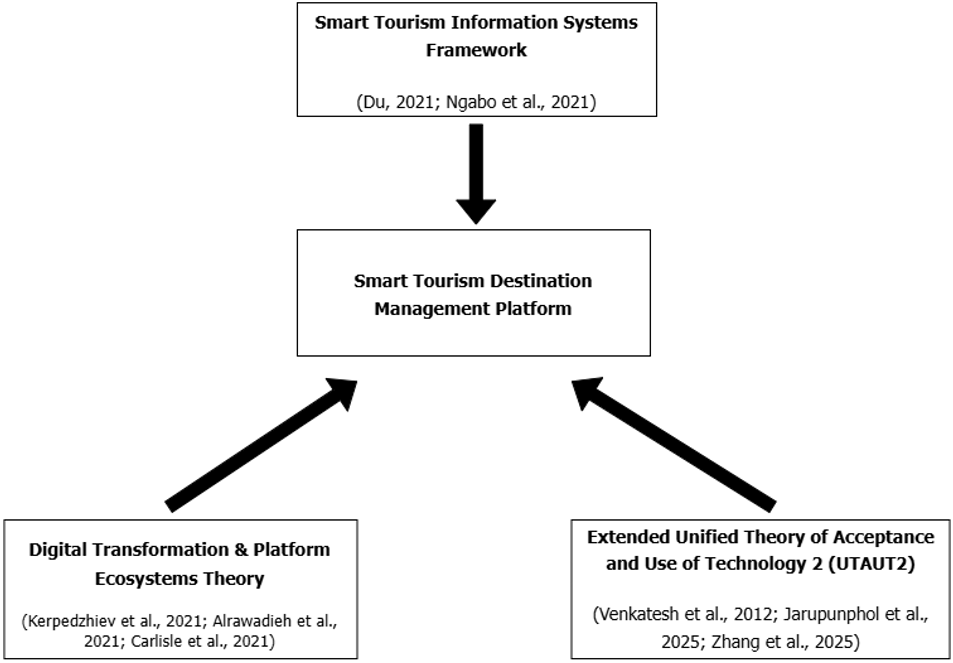
\includegraphics[width=1\textwidth]{Theoretical.png}
    \caption{Theoretical Paradigm}
    \label{fig:example}
\end{figure}

\section{Conceptual Framework}

This conceptual framework, structured on the standard Input-Process-Output-Outcome (IPOO) model, visually and logically maps the research for designing and analyzing a Smart Tourism Destination Management Platform.

\begin{figure}[h]
    \centering
    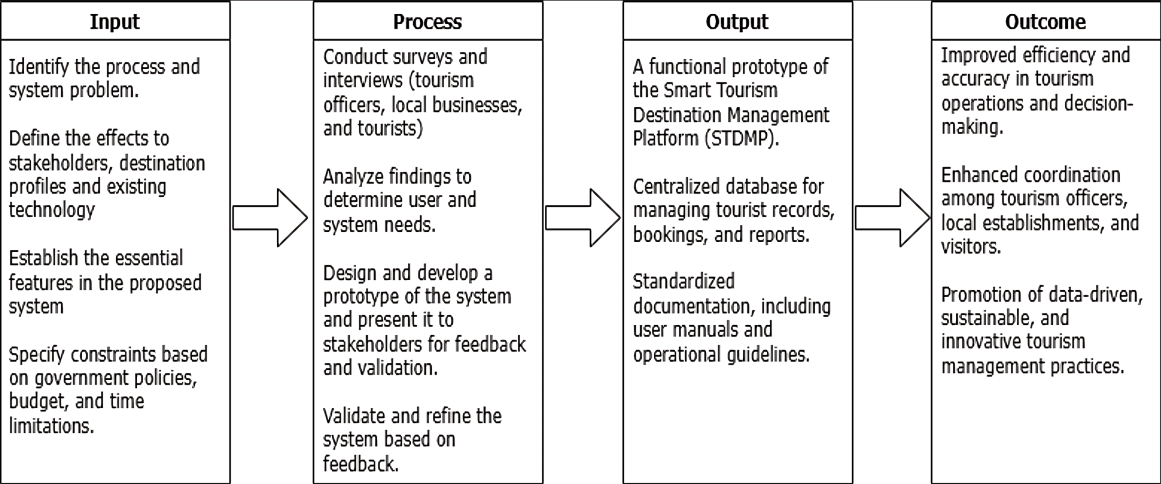
\includegraphics[width=1\textwidth]{ipoo_framework.png}
    \caption{Conceptual Paradigm}
    \label{fig:example}
\end{figure}

The Input phase addresses core organizational failures: process and system problems stemming from fragmented data and manual operations, which cause a lack of real-time reporting. This is contextualized by defining the effects on stakeholders, the specifics of destination profiles, and the limitations of existing technology. The scope is strictly managed by constraints such as government policies, budget, and time.

The Process phase details the methodology to create the solution. This involves gathering empirical data through surveys and interviews with tourism officers, local businesses, and tourists. These findings are analyzed to finalize user and system needs, which guide the design and development of a prototype. The final step is validation and refinement based on stakeholder feedback to ensure the system is practical and meets requirements.

The Output is a functional Smart Tourism Destination Management Platform prototype with a centralized database and standardized documentation. The ultimate Outcome is the realization of organizational benefits: improved efficiency and accuracy, enhanced coordination among tourism partners, and the promotion of data-driven, sustainable, and innovative tourism management practices.

\section{Statement of the Problem}

The main problem of the study is the design and development of a smart tourism destination management platform. Specifically, the study seeks to answer the following questions:

\begin{enumerate}
    \item What is the current state of and issues encountered in tourism management in Naga City?
    \item What smart tourism management platform could be designed and developed to enhance the tourism experience in Naga City?
    \item What is the level of usability, functionality, reliability, and security of the smart tourism management platform?
\end{enumerate}

\section{Assumptions}

The research was done based on the following assumptions, which are deemed necessary for ensuring consistency, relevancy, and credibility in conducting the research and developing the suggested platform.

\begin{enumerate}
    \item There are specific operational weaknesses and problems concerning the availability of information, promotional activities, tourism management, and coordination among tourism stakeholders in the current tourism management practices of Naga City, which can be studied and documented by conducting surveys, interviews, and other relevant methods.
    \item It is possible to develop the smart tourism management platform using the available technology in the context of Naga City, and such platform may help in managing tourism information, vouchers, promoting activities, and providing communication tools for improving tourism services and coordination.
    \item The measures and standards used for assessing the proposed smart tourism management platform, especially when it comes to usability, functionality, reliability, and security, can be considered suitable criteria for evaluating the proposed system prototype, and the participants who will take part in the assessment process will be able to give credible opinions about the proposed platform.
\end{enumerate}

\section{Scope and Delimitation}

The objective of this research is to design and develop a web-based Smart Tourism Destination Management Platform called BYANAGA for Naga City, Camarines Sur. The platform attempts to solve three operational issues: (1) there is no unified platform where tourists can discover vouchers and promotions; (2) there is no established online digital promotion system for the local tourism businesses; and (3) disorganized coordination between the Naga City Tourism Office and the private tourism industry.

There are four distinct user roles in this platform. Tourists have an ability to create a user account, view establishment profile cards that contain the title, description, picture, and voucher badge, explore available vouchers, make use of them at registered establishments utilizing vouchers' unique codes, etc. Owners can also register business accounts, submit documents, maintain and update their profiles when approved, add and publish events, create and submit vouchers, edit/cancel vouchers awaiting for approval, check all created vouchers depending on their current statuses, get revision feedbacks, confirm tourists' voucher redemption actions in the Redemption Panel, as well as see their performance metrics like total number of vouchers used and visitors foot traffic. Tourism officer's responsibilities include approving registration of establishments, vouchers' checking and feedback providing, event management, encoding tourists' arrivals, and tourism report generation and exporting. Administrator's role involves management of all user accounts, monitoring analytics and key performance indicators dashboards for the whole city, accessing audit trail, data backup management, etc.

The research is delimited by the following parameters. First, the platform is created and analyzed as a web application alone, while mobile app development is out of the scope and considered for future research. Second, the participants are purposively chosen from the population of Naga City, and therefore generalizability to other settings is not assumed. Third, the platform is assessed using SUS and UAT on a prototype basis only, and its evaluation in practice remains beyond the present scope. Fourth, the platform lacks third-party payment gateway support, and vouchers serve as online discount certificates used offline at participating businesses. Fifth, the administrator feature is included in the platform but validated through expert review.

\section{Significance of the Study}

BYANAGA assists in the digitalization of Naga City’s tourism industry by helping fill gaps in promotion distribution, establishment-to-tourist connection, and tourism management, which have been identified as factors currently hindering the city’s competitiveness in the tourism industry.

To Tourists and the Public in General. BYANAGA offers a one-stop solution for tourists visiting Naga City who want to find promotions and vouchers offered by all of the city’s registered establishments. Tourists can now look into promotions without the hassle of going through various sources. Event listings will also assist tourists in planning their visit according to the cultural and business events in the city.

For Establishment Owners and Small Businesses. BYANAGA enables small tourism businesses to have equal opportunities in terms of a structured digital promotional channel that was not available before. Regardless of their budget constraints, registration in BYANAGA enables small and medium tourism business owners to participate in a digital promotional process governed by the tourism office where tourists can be reached, tracked, and analyzed, providing more balanced promotional opportunities and contributing to overall economic development in the region.

For the Naga City Tourism Office and Local Government Unit. BYANAGA shifts the position of the tourism office personnel from mere coordination to governance through the use of a platform. The platform makes it possible to have standardized procedures in establishing businesses, approving vouchers, managing events, and encoding visitors' data. The platform facilitates decision-making based on data analysis in developing tourism strategies consistent with the NEDA Bicol Regional Development Plan [42] and DOT digitalization mandate [54]. Moreover, the platform contributes to Sustainable Development Goal (SDG) 8, 9, 11, and 17.

Recommendations for Further Researchers and System Developers. This research paper offers an adaptable template for creating online tourist destination portals within secondary cities in the Philippines and proves that digital transformation in local tourism governance can be accomplished without smart city infrastructure investment. The multi-agent design, voucher processing system led by officials, and multiple instrument assessment methods are replicable among other fragmented cities.

\section{Definition of Terms}

The following terms are defined as they are specifically applied to the design, development, and evaluation of the Smart Tourism Destination Management Platform for Naga City.

\textit{Administrator.} The user role in BYANAGA responsible for system-wide oversight, including management of all user accounts across all roles; monitoring city-wide analytics and KPI dashboards; access to the full audit trail and security logs; management of data backups and restore operations; and configuration of all system-wide settings and notification rules.

\textit{Appproval Queue.} The interface within the Tourism Officer panel displaying all pending establishment registration applications and submitted vouchers awaiting review. The officer processes each item by either approving or sending revision feedback with written notes specifying required changes.

\textit{Centralized Database.} A single, integrated data repository where all tourism-related records—including establishment profiles, voucher submissions, redemption logs, visitor arrival data, event listings, user accounts, notifications, and audit trails—are stored, organized, and accessed across all four user roles to eliminate data fragmentation.

\textit{Foot Traffic Data.} Visitor presence and movement data generated through BYANAGA's redemption confirmation records and profile engagement logs, providing establishment owners and the tourism officer with insights into visitor distribution patterns across registered establishments and time periods.

\textit{Fragmented Data.} Tourism records and information scattered across multiple files, offices, or systems, resulting in inconsistencies and difficulties in generating complete and timely reports prior to the introduction of the centralized platform.

\textit{User Acceptance Testing (UAT).} The formal evaluation phase in which actual end-users, such as tourism officers and partner businesses, use the prototype to verify whether its features, usability, and performance meet practical requirements.

\textit{Centralized Database.} A single, integrated repository within the platform where all tourism-related data from different sources are stored, organized, secured, and accessed to eliminate duplication and fragmentation.

\textit{Tourist.} A registered user of the BYANAGA platform who browses establishment profiles, discovers available vouchers and promotions from all registered Naga City establishments in a single website, and redeems vouchers at registered establishments by presenting the unique voucher code at the Redemption Panel.

\textit{Tourism Officer.} The user role in BYANAGA representing the Naga City Tourism Office staff member responsible for platform governance. The tourism officer reviews establishment registration applications, approves or sends revision feedback on voucher submissions, manages city-wide events, encodes visitor arrival records, generates tourism reports, and monitors platform analytics.

\textit{User Acceptance Testing (UAT).} A formal evaluation phase in which actual end-users—tourists, establishment owners, and the tourism officer—interact with the functional BYANAGA prototype by performing defined role-specific tasks. UAT verifies that the platform's features, usability, and performance meet the practical workflow requirements of each user role.

\textit{Voucher.} A digital promotional offer created and submitted by an Establishment Owner through BYANAGA, reviewed and approved by the Tourism Officer, and published to tourists on the platform. Each approved voucher carries a unique redemption code. Voucher statuses are: Pending, Revision, or Approved.

\clearpage

%-----------------------------
% Chapter 2
%-----------------------------
\chapter{Methods}

\section{Research Design}
The proposed research will use a developmental research design that is best suited for studies that involve the design, implementation, and systematic evaluation of an information system [89]. In this regard, the developmental model will dictate the systematic process of building BYANAGA from the identification of the system requirements and design through the prototyping and evaluation of its usability and performance with real users. The quantitative data collected using SUS and the performance test metrics will be used to determine the technical usability and efficiency of the platform, while qualitative data collected through the open-ended surveys and UAT will provide insights on user requirements and interface challenges.

\section{Respondents and Sampling}

The respondents of the study were composed of those who have participated in tourism operations and tourism-related services in Naga City. Purposive sampling was done when choosing the respondents since they have been selected based on their relevance to the study and their experience with tourism.

A total of thirty-six (36) respondents were identified in conducting the interviews. There were thirty (30) tourists, five (5) establishment owners, and one (1) tourism officer from the Local Government Unit of Naga City as respondents. The thirty (30) tourists were made up of people who had been, were, or had any knowledge of the tourism services within Naga City. They were considered respondents since they were essential in providing data on the common problems encountered during their searches for tourism information and plans.

Five (5) establishment owners served as respondents for the purposes of gathering data on their tourism operations and experiences in the tourism industry.

The tourism officer respondents are from the Local Government Unit Tourism Office and offered information concerning administration and operations in relation to monitoring of tourism, managing of tourism data, reporting and decision making in tourism. Inclusion of such respondents in the study made it possible for the project to acquire the required operational and end-user views.

\section{Data gathering Procedure}

The data collection methodology involved a systematic three-step approach guaranteeing complete data collection for both qualitative and quantitative data at all levels of platform development and evaluation.

Step 1 – Problem Identification and Requirement Gathering. The first step in the data collection methodology involved establishing the baseline by conducting: (a) interviews with the Tourism Officer of the Naga City DMO to determine the processes used, pain points, and governance requirement for vouchers and establishments; (b) survey questionnaires sent to the establishment owner and tourists on a 5-point Likert Scale asking open-ended questions about their current method of discovery and their requirements for the platform; and (c) observations conducted at the DMO and analysis of tourism documents available to determine the constraints influencing the design requirements of the platform.

Phase 2 — Design and Development of the System. With respect to the findings in Phase 1, the design and development of BYANAGA was carried out as outlined in Section 2.6. In this regard, all four role-based interfaces and related systems such as centralized database, voucher submission and approval system, voucher redemption confirmation system, and analytics/reporting system were designed. Various system documentation documents that include Data Flow Diagram (DFD), Business Process Modeling Notation (BPMN), and Entity Relationship Diagram (ERD) were prepared as part of system design and development.

Phase 3 — Prototype Evaluation (Validation, Testing, and Feedback). Following the development of the prototype of the platform, a two-step process of evaluation was followed. Firstly, expert validation was carried out with an IT panel consisting of IT experts and academicians who were supposed to validate the overall design of the platform and data flows. Secondly, UAT was undertaken for all three respondent groups, where each user performed role-specific operations on the functioning prototype of BYANAGA. Afterwards, SUS test was undertaken, along with other feedback mechanisms from UAT and focus groups.

\section{Research Instrument}
Survey Questionnaire. Conducted during Phase 1 among establishment managers and tourists. The questionnaire consisted of closed-ended questions using the Likert scale assessing current promotional discovery practices and feature importance rankings, along with open-ended questions aimed at collecting qualitative insights regarding operational issues and user expectations. It served as the starting point for system requirement definition.

Interview Guide Questionnaire. Semi-structured interview guide designed to facilitate in-depth interviews with the Tourism Officer during Phase 1. The guide was used to understand current DMO processes and inefficiencies associated with them, as well as to determine requirements for the governance aspects of the portal, such as the approval and feedback systems.

System Usability Scale (SUS). Used on all three sets of respondents after the UAT phase in Phase 3. The ten items on the SUS questionnaire allow users to indicate the level of usability in terms of ease of learning, efficiency, and satisfaction [65]. Three different SUS questionnaires were administered for tourists, establishment owners, and tourism officers.

Performance Metrics Evaluation Tool. Structured tool used for the technical evaluation of the system in the third phase to determine important metrics like average page load time, data processing time, voucher process time, reports time, and system behavior under simulated multi-user environments.

\section{Ethical Considerations}

Proper ethical considerations were made when implementing the research study. It should be noted that participation in the research study was voluntary for all the respondents, and they were informed about the objectives of the research study before involving them in the research study. Forms were provided to all the respondents in which consent was sought from them before starting the research study.

All the respondents were informed that their information would remain confidential, and the data collected would only be used for research purposes. It is also necessary to state that all the respondents had the freedom not to respond to the survey questions or even withdraw from the research study without any repercussions. All the procedures of the research study adhered to the provisions of the Data Privacy Act of 2012 (Republic Act No. 10173).

\section{Statistical Treatment of Data}
Statistical analysis using descriptive statistics was used to analyze the quantitative data collected through the questionnaire survey. The frequency and percentage distribution were used to describe the profile of the respondents. Weighted mean was used to ascertain the respondents' perceptions on the existing tourism management system, technological constraints, usefulness of the proposed BYANAGA platform, and intention of adopting the same.

These weighted means were analyzed using the five-point scale interpretation ranging from 'Strongly Disagree' to 'Strongly Agree.' Through these statistical techniques, the researchers could effectively analyze the data collected from the respondents.

\section{System Design and Architecture}

The BYANAGA Smart Tourism Destination Management Platform supports four different roles for users on one integrated web-based system in Naga City. These include centralized promotions discovery for the tourists, provision of establishment owners with a digital promotion mechanism under the governance of the tourism officer, and the administrator's access to full system control. It comprises three layers, namely, Presentation Layer that implements the web-based interfaces with differentiated functionality for each of the four users, Application Layer responsible for implementing the entire logic such as voucher transactions, approval queue, redemption status, analysis calculation, and reporting, and the Data Layer that ensures the storage in a persistent fashion via relational database comprising tables for establishments, vouchers, redemptions, events, arrivals, users, notifications, and logs.

\subsection{Data Flow Diagram}
A Data Flow Diagram (DFD) was created to give a visualization of how data flow occurs on BYANAGA from external entities through internal processes to storage. The four external entities, namely Tourist, Establishment Owner, Tourism Officer, and Administrator, interact with BYANAGA by inputting and getting outputted data respectively at the context level (Level 0). At Level 1, the DFD illustrates how the entire system is broken down to five fundamental sub-processes including: (1) User Authentication and Account Management; (2) Establishment Profile and Content Management; (3) Voucher Submission and Approval Process; (4) Voucher Redemption and Analysis Process; and (5) Administration and System Monitoring. Every process that takes place within the sub-processes is logged on the audit record data store.

\subsection{Business Process Modeling Notation (BPMN)}
By using the Business Process Modeling Notation (BPMN), major processes in BYANAGA were modeled to achieve an easy-to-understand graphical representation of processes in terms of actions, decisions, events, and interactions among them [91]. BPMN was chosen as a modeling tool due to its standardized visual form which makes the validation of the process easier by both the technical development team and non-technical personnel, including tourism officers and owners of establishments, through the use of expert evaluation technique. The major processes that were captured via BPMN include four processes: (1) Establishment Registration and Approval Process, (2) Voucher Submission, Review, and Publication Process, (3) Tourist Voucher Discovery and Redemption Process, and (4) Tourism Officer Reporting and Visitor Data Encoding Process.

\subsection{Entity-Relationship Diagram}
To represent the database design of BYANAGA, an Entity Relationship Diagram (ERD) was created [92]. According to the diagram, there are eight main entities that were used during the database design process: User (there are four roles in total with role being the attribute of the entity); Establishment (with profile attributes, registration status, establishment owner); Voucher (connected to the establishment, with status attribute, redemption code, revision history); Redemption (every single redemption of the voucher, connected to the tourist and voucher; timestamp); Event (linked to an establishment; can be posted independently by the tourism officer); Visitor Record (visitor’s visitation recorded by the tourism officer); Notification (linked to user and related to the notifications sent from the system); and Audit Log (records every activity performed by an admin).

\subsection{Tourist Interface}
Tourist Interface is the user interface of BYANAGA that will allow tourists visiting Naga City to have access to all the promotional activities done by the city’s establishments and tourism officer through one single website. Establishment Listings are displayed as visual cards containing the name of the establishment, category, description, images, and badges if any voucher is available. Tourists can filter and search establishments using the filters or keywords. Voucher Discovery Page shows a list of all active and approved vouchers offered by all the registered establishments. Each visual card consists of the name of the establishment, voucher name, description, terms and conditions, and validity period. Once the tourist clicks on a voucher, he or she will receive a unique code for presenting the same at the establishment. Events Page shows a list of upcoming events organized by establishment owners and the tourism officer. Tourist Account Page enables the tourists to update their profile and redeeming history.

\subsection{Establishment Owner Interface}
The Establishment Owner Interface is an effective management tool provided to local businesses that are registered. The Registration and Profile Setup module walks owners of the establishment through submitting documents, which include business permits and owner identification documents, while monitoring the process of registration and approval status through the queue of the officer. Upon completion, the Business Profile Manager helps owners change the description of the establishment, contact information, opening hours, price range, and image gallery, which become part of the establishment card used by tourists. The Voucher Management Module offers a chance for owners to create vouchers including title, description, discount, validity period, and conditions, after which the vouchers go into the queue for officer approval. The vouchers are monitored by their status - Pending, Revision, and Approved – and are editable or removable in case of a pending voucher. Owners can review the notes given during revision and make corrections to the voucher before sending it back to the officer. The Redemption Panel allows the staff to check the tourist vouchers entered according to the code provided.

\subsection{Tourism Officer Interface}
The Tourism Officer Interface acts as the governance board of BYANAGA. The Validation Queue consists of all the pending application submissions from establishments for registration; the officer can either approve the submission, which will make the profile live, or provide revision feedback asking for more supporting documents. The Voucher Review Queue is the queue of all the submitted vouchers awaiting approval; the officer can either approve the voucher, which will make it instantly viewable by tourists, or give revision feedback along with written notes. The system does not allow any form of rejection, maintaining a positive working relationship with the owners of the businesses [26]. The Event Management Module lets the officer create and manage events that will be taking place around the city related to tourism, while also giving the officer access to the event submissions made by establishment owners. The Visitor Data Encoding Module allows for an organized interface for the input of the visitor arrivals' details, which comes with error detection capabilities.

\subsection{Administrator Interface}
Administrator Interface will facilitate overall system management and configuration. User Management Module will help in account management, such as creating accounts for officers and allocating their roles, approving establishments at the system level, and also management of tourist accounts. City-Wide Analytics Dashboard will display consolidated statistics including total registration numbers, number of vouchers, volume of voucher redemptions, visitors statistics, and KPI achievements according to predefined targets. Voucher Analytics will display statistics of promotional activities across establishments. Audit Trail module will provide an exhaustive log of all actions performed in the system. Security and Access Logs will display logins as well as other security-related notifications. System Configuration module will handle system configuration, backups and restoration processes, and other tasks including defining of notification rules and workflow approval configurations.

\section{Validation and Testing Methods}
Expert Validation. Before the users' acceptance testing process, the BYANAGA prototype went through expert validation by an evaluation panel comprising IT experts, system developers, and academic advisors. The panel assessed the system architecture of the platform, the interfaces designs for all the four user types, data flow diagrams, BPMN models, and ERD based on the aspects of functionality, reliability, security, and design integrity.

User Acceptance Testing (UAT). After expert validation, user acceptance testing was done using the three respondent types. Each type was assigned task-specific responsibilities, which were completed accordingly. Tourists were required to do establishment browsing tasks, voucher search tasks, and voucher redemption tasks. Establishment owners had to carry out establishment profile set-up tasks, submit vouchers, respond to any revisions requested, and confirm the voucher redemption process. Finally, the tourism officer had to accomplish establishment approval tasks, review vouchers, organize events, encode visitors' information, and generate reports.

Performance and Accuracy Testing. The technical testing evaluated the efficiency of the application during actual use, documenting such parameters as the time taken to load pages, time response for processing vouchers, time taken to generate reports, data retrieval speed, and performance of the system during simulations of multiple user sessions. Accuracy tests checked the consistency of data on voucher details, redemption of the vouchers, and data about the visitors from all the interfaces provided. The data was expected to be consistent even if changes were made from any of the user perspectives.

Feedback Analysis and Refinements. Quantitative data collected from SUS surveys and performance testing was analyzed using descriptive statistical tools while qualitative feedback received through UAT observation and SUS survey comments and focused group discussion with DMO officers and business owners was analyzed for themes.

\chapter{Results and Discussions}

\section{Results}

\subsection{Problem 1: Current State and Issues Encountered in Tourism 
Management in Naga City}

This section presents the results of the survey conducted among thirty (30) tourist 
respondents and five (5) establishment owner respondents to document the current 
state of tourism management in Naga City and identify the specific problems and 
inefficiencies that motivated the development of BYANAGA. The findings are 
organized according to respondent group and survey section.

\subsubsection{Tourist Respondents}

\paragraph{Respondent Profile}

\begin{table}[h]
    \centering
    \begin{tabular}{|l|c|c|}
        \hline
        \textbf{Travel Experience} & \textbf{Frequency} & \textbf{Percentage} \\
        \hline
        First-time Visitors & 16 & 53.33\% \\
        Repeat Visitors     & 14 & 46.67\% \\
        \hline
        \textbf{Total} & \textbf{30} & \textbf{100\%} \\
        \hline
    \end{tabular}
    \caption{Travel Experience of Tourist Respondents}
    \label{tab:travel_experience}
\end{table}

Table~\ref{tab:travel_experience} presents the distribution of travel experience 
among the thirty (30) tourist respondents. The majority were first-time visitors 
to Naga City, comprising 53.33\% of the total, while repeat visitors accounted 
for 46.67\%. This near-equal distribution is significant for the development of 
BYANAGA. First-time visitors, lacking prior familiarity with Naga City's tourism 
offerings, are most dependent on a centralized platform to discover available 
promotions, establishments, and vouchers. Repeat visitors, on the other hand, 
represent a segment that has already experienced the fragmented information 
landscape and stands to benefit directly from the organizational convenience that 
BYANAGA provides. The near-equal split between both groups confirms that the 
platform must simultaneously serve the discovery needs of new visitors and the 
convenience expectations of returning ones.

\begin{table}[h]
    \centering
    \begin{tabular}{|l|c|c|}
        \hline
        \textbf{Travel Group} & \textbf{Frequency} & \textbf{Percentage} \\
        \hline
        Solo       & 8  & 26.67\% \\
        Family     & 6  & 20.00\% \\
        Friends    & 10 & 33.33\% \\
        Group Tour & 6  & 20.00\% \\
        \hline
        \textbf{Total} & \textbf{30} & \textbf{100\%} \\
        \hline
    \end{tabular}
    \caption{Travel Group Composition of Tourist Respondents}
    \label{tab:travel_group}
\end{table}

Table~\ref{tab:travel_group} shows the travel group composition of the tourist 
respondents. The largest proportion traveled with friends (33.33\%), followed 
by solo travelers (26.67\%), while family groups and organized group tours each 
accounted for 20.00\%. The combined dominance of friend-group and solo travelers 
at 60\% of total respondents indicates that the majority of tourists visiting Naga 
City make relatively independent and self-directed travel decisions. These traveler 
types are less likely to rely on pre-arranged tour packages and more likely to seek 
real-time, self-service digital tools for discovering deals, planning their itinerary, 
and choosing which establishments to visit. This finding directly supports 
BYANAGA's tourist-facing features — including the establishment browsing 
interface, voucher discovery page, personal itinerary builder, and wishlist — as 
these are precisely the tools that independent travelers use to organize and 
optimize their visits without the guidance of a tour coordinator.

\begin{table}[h]
    \centering
    \begin{tabular}{|l|c|c|}
        \hline
        \textbf{Length of Stay} & \textbf{Frequency} & \textbf{Percentage} \\
        \hline
        Day Trip    & 16 & 53.33\% \\
        1--3 Nights & 10 & 33.33\% \\
        4+ Nights   & 4  & 13.33\% \\
        \hline
        \textbf{Total} & \textbf{30} & \textbf{100\%} \\
        \hline
    \end{tabular}
    \caption{Length of Stay of Tourist Respondents}
    \label{tab:length_stay}
\end{table}

Table~\ref{tab:length_stay} reveals that more than half of tourist respondents 
(53.33\%) were day-trip visitors, followed by those staying one to three nights 
(33.33\%), and a small minority staying four or more nights (13.33\%). The 
dominance of day-trip visitors carries significant implications for the design 
priority of BYANAGA. A tourist spending only a few hours in Naga City has an 
extremely limited window to discover, evaluate, and claim available promotions. 
Under the current fragmented landscape --- where deals are scattered across 
multiple websites and social media platforms --- a day-trip visitor is most likely 
to miss promotional opportunities entirely due to the time cost of the discovery 
process. This finding directly validates BYANAGA's core value proposition: 
consolidating all available Naga City vouchers, promos, and establishment 
information into a single website that a tourist can access immediately upon 
arrival. The shorter the visit duration, the greater the impact of a centralized 
platform on the tourist's ability to maximize their experience.

\begin{table}[h]
    \centering
    \begin{tabular}{|l|c|c|}
        \hline
        \textbf{Main Interest} & \textbf{Frequency} & \textbf{Percentage} \\
        \hline
        Attractions  & 10 & 33.33\% \\
        Food/Promos  & 8  & 26.67\% \\
        Culture      & 7  & 23.33\% \\
        Shopping     & 5  & 16.67\% \\
        \hline
        \textbf{Total} & \textbf{30} & \textbf{100\%} \\
        \hline
    \end{tabular}
    \caption{Primary Tourist Interests of Respondents}
    \label{tab:tourist_interests}
\end{table}

Table~\ref{tab:tourist_interests} shows that physical attractions ranked as the 
primary interest of tourist respondents (33.33\%), followed closely by food and 
promotions (26.67\%), culture (23.33\%), and shopping (16.67\%). The strong 
second-place showing of food and promotions as a primary travel motivator is 
particularly relevant to BYANAGA's purpose. More than one in four tourists 
identified food and promotional deals as their main reason for visiting --- a 
figure that confirms promotional offers are not merely a secondary convenience 
but a genuine driver of tourist decision-making and destination choice. When 
combined with the cultural interest category (23.33\%), which frequently includes 
local food experiences in the Philippine context, the centrality of food tourism 
to Naga City's visitor market becomes even more apparent. These findings reinforce 
the appropriateness of BYANAGA's voucher and promotion discovery system as a 
primary platform feature rather than a supplementary one.

\paragraph{Current Problems and Impacts}

\begin{table}[h]
    \centering
    \begin{tabular}{|l|c|c|}
        \hline
        \textbf{Statement} & \textbf{Weighted Mean} & \textbf{Interpretation} \\
        \hline
        Too many websites/social media to check for deals & 3.97 & Agree \\
        Promos expire before I can find and reach them    & 4.00 & Agree \\
        Language barriers on local menus/offers           & 3.60 & Agree \\
        Hard to combine deals across categories           & 4.10 & Agree \\
        \hline
        \textbf{Overall Weighted Mean} & \textbf{3.92} & \textbf{Agree} \\
        \hline
    \end{tabular}
    \caption{Current Problems and Impacts Experienced by Tourist Respondents}
    \label{tab:tourist_problems}
\end{table}

Table~\ref{tab:tourist_problems} presents the tourist respondents' ratings of 
current problems encountered when searching for and accessing tourism promotions 
in Naga City, yielding an overall weighted mean of 3.92 interpreted as Agree. 
The highest-rated problem was the difficulty of combining deals across 
restaurants, transport services, and attractions (M=4.10), indicating that 
tourists are not merely inconvenienced by scattered information --- they are 
actively unable to maximize their travel value because no mechanism exists to 
cross-reference and bundle multiple promotional offers in one place. This finding 
is the most direct validation of BYANAGA's multi-establishment voucher 
aggregation feature.

The second-highest rated problem was promotional expiry before discovery 
(M=4.00), which reflects a real and recurring economic cost for tourists: deals 
that exist but cannot be found in time are functionally equivalent to deals that 
do not exist at all. This aligns closely with the day-trip visitor dominance 
identified in Table~\ref{tab:length_stay}, as shorter visit durations compound 
the urgency of timely promotional discovery. The burden of monitoring too many 
websites and social media channels (M=3.97) received a nearly identical rating, 
confirming that the problem is not a lack of digital promotional content but its 
structural fragmentation across too many platforms. Language barriers on local 
menus and offers, while the lowest-rated item (M=3.60), still received an Agree 
interpretation, identifying it as a secondary but genuine obstacle for non-local 
tourists engaging with Naga City's establishments.

\paragraph{Technological Gaps}

\begin{table}[h]
    \centering
    \begin{tabular}{|l|c|c|}
        \hline
        \textbf{Statement} & \textbf{Weighted Mean} & \textbf{Interpretation} \\
        \hline
        Need GPS-linked promo map showing nearby deals   & 4.27 & Strongly Agree \\
        Want offline access to saved Naga City offers    & 4.40 & Strongly Agree \\
        Current apps do not filter deals by budget/time  & 3.87 & Agree          \\
        No way to see promo reviews from recent visitors & 4.33 & Strongly Agree \\
        Wish for QR code scanning for instant deals      & 4.53 & Strongly Agree \\
        \hline
        \textbf{Overall Weighted Mean} & \textbf{4.28} & \textbf{Strongly Agree} \\
        \hline
    \end{tabular}
    \caption{Technological Gaps Identified by Tourist Respondents}
    \label{tab:tourist_tech_gaps}
\end{table}

Table~\ref{tab:tourist_tech_gaps} presents tourist respondents' assessments of 
specific digital tool gaps in the current Naga City tourism landscape, producing 
an overall weighted mean of 4.28 interpreted as Strongly Agree --- the 
second-highest rated section among tourist respondents. The highest-rated gap 
was the desire for QR code scanning at venues for instant deal access (M=4.53), 
which directly aligns with BYANAGA's unique voucher code redemption mechanism, 
where tourists receive a unique code per claimed voucher that is confirmed by 
establishment staff through the Redemption Panel.

The desire for offline access to saved offers (M=4.40) reflects practical 
connectivity limitations tourists may encounter while visiting establishments. 
BYANAGA's wishlist and saved voucher features address this need by allowing 
tourists to save relevant promotions before they arrive at an establishment. The 
absence of a reliable review and rating system for promotions and establishments 
(M=4.33) directly supports BYANAGA's post-redemption review feature, which 
enables tourists to rate and review an establishment after a confirmed voucher 
redemption. The need for a location-aware promotional map (M=4.27) reflects 
tourists' desire for proximity-based discovery --- a feature identified as a 
future development direction for BYANAGA. The finding that current applications 
fail to filter deals by budget or time (M=3.87), while the lowest-rated item, 
still falls in the Agree range and supports the search and filter functionality 
built into BYANAGA's voucher discovery interface.

\paragraph{Filipino Dish and Food Bundle Interest}

\begin{table}[h]
    \centering
    \begin{tabular}{|l|c|c|}
        \hline
        \textbf{Response} & \textbf{Frequency} & \textbf{Percentage} \\
        \hline
        Yes & 27 & 90.00\% \\
        No  & 3  & 10.00\% \\
        \hline
        \textbf{Total} & \textbf{30} & \textbf{100\%} \\
        \hline
    \end{tabular}
    \caption{Interest in Filipino Dishes Among Tourist Respondents}
    \label{tab:filipino_dish_tourist}
\end{table}

Table~\ref{tab:filipino_dish_tourist} reveals that 90.00\% of tourist respondents 
expressed interest in trying Filipino dishes during their visit to Naga City, 
with only 10.00\% indicating otherwise. This near-unanimous interest underscores 
the centrality of local culinary experience to the Naga City tourist visit and 
directly establishes food tourism as a primary engagement driver for the 
platform's establishment directory. The Bicol Region's distinct culinary 
identity --- anchored by signature dishes such as Bicol Express, Laing, and 
Pinangat --- represents a powerful and differentiated tourist attraction that 
local food and dining establishments can leverage through BYANAGA's promotional 
voucher system.

\begin{table}[h]
    \centering
    \begin{tabular}{|l|c|c|}
        \hline
        \textbf{Response} & \textbf{Frequency} & \textbf{Percentage} \\
        \hline
        Yes       & 22 & 73.33\% \\
        Sometimes & 4  & 13.33\% \\
        No        & 4  & 13.33\% \\
        \hline
        \textbf{Total} & \textbf{30} & \textbf{100\%} \\
        \hline
    \end{tabular}
    \caption{Interest in Food Bundle Promotions Among Tourist Respondents}
    \label{tab:food_bundle_tourist}
\end{table}

Table~\ref{tab:food_bundle_tourist} shows that 73.33\% of tourist respondents 
actively seek food bundle promotions when visiting a destination, with an 
additional 13.33\% doing so occasionally. Cumulatively, 86.66\% of tourist 
respondents demonstrated a positive disposition toward bundled promotional 
offers. This finding confirms that bundled promotional mechanics --- where a 
single voucher provides value across multiple items or services --- are the 
preferred promotional format among the majority of the tourist respondent pool, 
directly validating the bundle-capable voucher design within BYANAGA's 
establishment owner portal. Furthermore, it establishes that food bundle 
promotions function as a visit motivator: tourists who are already planning to 
visit are more likely to choose specific establishments when a promotional bundle 
is available, reinforcing the urgency of providing establishment owners with a 
streamlined tool for publishing bundle-type vouchers.

\paragraph{AI Integration Potential}

\begin{table}[h]
    \centering
    \begin{tabular}{|l|c|c|}
        \hline
        \textbf{Statement} & \textbf{Weighted Mean} & \textbf{Interpretation} \\
        \hline
        AI shows deals matching taste and current location & 4.70 & Strongly Agree \\
        Voice search for nearby local deals               & 4.37 & Strongly Agree \\
        AI warns if better deals exist before I commit    & 4.80 & Strongly Agree \\
        Chatbot answers promo-specific questions          & 4.43 & Strongly Agree \\
        AI builds personalized 1-day Naga itinerary       & 4.67 & Strongly Agree \\
        \hline
        \textbf{Overall Weighted Mean} & \textbf{4.59} & \textbf{Strongly Agree} \\
        \hline
    \end{tabular}
    \caption{AI Integration Potential as Rated by Tourist Respondents}
    \label{tab:tourist_ai}
\end{table}

Table~\ref{tab:tourist_ai} presents tourist respondents' ratings of proposed 
AI-powered features, yielding an overall weighted mean of 4.59 --- the 
highest-rated section across all tourist survey categories, interpreted as 
Strongly Agree. This result indicates that respondents do not merely accept 
AI-powered tourism features as optional enhancements but regard them as strongly 
desirable and expected capabilities of a modern tourism platform.

The highest-rated feature was AI notifications alerting tourists when better 
deals exist before they commit to a current offer (M=4.80), reflecting a 
sophisticated consumer preference for deal optimization rather than simple 
discovery. Location-aware AI deal matching based on personal taste and proximity 
ranked second (M=4.70), confirming strong demand for personalized, context-sensitive 
promotional recommendations. AI-powered itinerary building (M=4.67), chatbot 
assistance for promo queries (M=4.43), and voice search (M=4.37) all received 
Strongly Agree ratings, demonstrating broad and consistent appetite for intelligent 
tourism assistance across multiple interaction modes. These findings collectively 
establish a clear direction for AI-enhanced feature development in future 
iterations of BYANAGA.

\paragraph{Platform Benefits for Better Tourism}

\begin{table}[h]
    \centering
    \begin{tabular}{|l|c|c|}
        \hline
        \textbf{Statement} & \textbf{Weighted Mean} & \textbf{Interpretation} \\
        \hline
        Track popular walking routes between deal locations & 4.57 & Strongly Agree \\
        Identify traffic hotspots around promo venues       & 4.73 & Strongly Agree \\
        Spot seasonal deal preferences for event planning   & 4.30 & Strongly Agree \\
        Map most-requested food types by neighborhood       & 4.27 & Strongly Agree \\
        Predict busy hours to staff promo locations better  & 4.67 & Strongly Agree \\
        \hline
        \textbf{Overall Weighted Mean} & \textbf{4.51} & \textbf{Strongly Agree} \\
        \hline
    \end{tabular}
    \caption{Perceived Platform Benefits for City-Wide Tourism Improvement (Tourist)}
    \label{tab:tourist_platform_benefits}
\end{table}

Table~\ref{tab:tourist_platform_benefits} presents tourist respondents' ratings 
of city-wide platform data benefits, yielding an overall weighted mean of 4.51 
interpreted as Strongly Agree. Notably, this section asks tourists to evaluate 
benefits that extend beyond personal convenience to the broader tourism 
ecosystem, and their strong agreement across all items indicates that respondents 
view a centralized tourism platform as a public good rather than merely a 
personal utility.

The highest-rated item was identifying traffic hotspots around promotional 
venues (M=4.73), followed by predicting busy hours for better staffing at 
promotional locations (M=4.67). These items reflect tourist awareness that 
platform data can improve the quality of their visit indirectly --- by enabling 
better resource management at the establishments and venues they patronize. 
Tracking popular walking routes between deal locations (M=4.57) confirms that 
tourists are interested in spatially organized promotional discovery. Spotting 
seasonal deal preferences for event planning (M=4.30) and mapping food type 
demand by neighborhood (M=4.27), while the lowest-rated items in this section, 
still received Strongly Agree interpretations, confirming that the full range of 
city-level data benefits proposed for BYANAGA are recognized and valued by the 
tourist respondent group.

\subsubsection{Establishment Respondents}

\paragraph{Respondent Profile}

\begin{table}[h]
    \centering
    \begin{tabular}{|l|c|c|}
        \hline
        \textbf{Establishment Type} & \textbf{Frequency} & \textbf{Percentage} \\
        \hline
        Restaurant    & 2 & 40.00\% \\
        Hotel         & 1 & 20.00\% \\
        Tour Agency   & 1 & 20.00\% \\
        Souvenir Shop & 1 & 20.00\% \\
        \hline
        \textbf{Total} & \textbf{5} & \textbf{100\%} \\
        \hline
    \end{tabular}
    \caption{Type of Establishment of Respondents}
    \label{tab:estab_type}
\end{table}

Table~\ref{tab:estab_type} presents the types of establishments represented 
among the five (5) establishment respondents. Restaurants comprised the largest 
single group at 40.00\%, with hotels, tour agencies, and souvenir shops each 
representing 20.00\%. The dominance of restaurants is consistent with the strong 
food tourism interest identified among tourist respondents in 
Tables~\ref{tab:filipino_dish_tourist} and~\ref{tab:food_bundle_tourist}, 
reflecting the outsized role of food and dining businesses in the Naga City 
tourism landscape. The hotel respondent is noted within the context of BYANAGA's 
design: while accommodation booking is not a platform feature, hotel 
establishments are included in the directory as informational profiles displaying 
contact details and descriptions for tourist inquiry purposes. The inclusion of 
tour agencies and souvenir shops confirms that BYANAGA's establishment category 
system represents the actual composition of Naga City's tourism business sector.

\begin{table}[h]
    \centering
    \begin{tabular}{|l|c|c|}
        \hline
        \textbf{Years of Operation} & \textbf{Frequency} & \textbf{Percentage} \\
        \hline
        1--3 Years  & 2 & 40.00\% \\
        4--10 Years & 2 & 40.00\% \\
        10+ Years   & 1 & 20.00\% \\
        \hline
        \textbf{Total} & \textbf{5} & \textbf{100\%} \\
        \hline
    \end{tabular}
    \caption{Years of Operation of Establishment Respondents}
    \label{tab:years_operation}
\end{table}

Table~\ref{tab:years_operation} shows that establishment respondents are 
distributed across varying levels of operational experience. Forty percent have 
operated for one to three years, another 40.00\% for four to ten years, and 
20.00\% for more than ten years. The presence of newer businesses is particularly 
relevant to BYANAGA's value proposition: establishments operating for one to 
three years are least likely to have developed established promotional channels 
or a loyal tourist following, making the platform's structured digital promotion 
infrastructure most impactful for this segment. More experienced establishments 
bring operational insight into the specific promotional coordination challenges 
that BYANAGA is designed to address, lending credibility to the problems 
identified in the subsequent survey sections.

\begin{table}[h]
    \centering
    \begin{tabular}{|l|c|c|}
        \hline
        \textbf{Number of Employees} & \textbf{Frequency} & \textbf{Percentage} \\
        \hline
        1--5 Employees   & 2 & 40.00\% \\
        6--20 Employees  & 2 & 40.00\% \\
        21--50 Employees & 1 & 20.00\% \\
        \hline
        \textbf{Total} & \textbf{5} & \textbf{100\%} \\
        \hline
    \end{tabular}
    \caption{Number of Employees of Establishment Respondents}
    \label{tab:num_employees}
\end{table}

Table~\ref{tab:num_employees} reveals that 80.00\% of establishment respondents 
are small to medium enterprises, employing between one and twenty staff members. 
Only 20.00\% employ between twenty-one and fifty workers, and none employ more 
than fifty. This workforce profile is directly relevant to the platform's design 
rationale: small businesses with one to five employees have extremely limited 
capacity for managing multiple digital promotion channels simultaneously. The 
time and resource cost of maintaining separate social media accounts, coordinating 
with tourism offices through informal channels, and manually tracking promotional 
redemptions represents a disproportionate burden for single-digit employee 
operations. BYANAGA's establishment owner portal --- which consolidates profile 
management, voucher creation, officer communication, and redemption tracking into 
one interface --- is most impactful precisely for this majority small-enterprise 
segment.

\paragraph{Filipino Dish and Food Bundle Offerings}

\begin{table}[h]
    \centering
    \begin{tabular}{|l|c|c|}
        \hline
        \textbf{Response} & \textbf{Frequency} & \textbf{Percentage} \\
        \hline
        Yes & 2 & 100.00\% \\
        No  & 0 & 0.00\%   \\
        \hline
        \textbf{Total} & \textbf{2} & \textbf{100\%} \\
        \hline
    \end{tabular}
    \caption{Filipino Dish Offerings Among Restaurant Respondents}
    \label{tab:filipino_dish_estab}
\end{table}

Table~\ref{tab:filipino_dish_estab} shows that all restaurant respondents 
(100.00\%) confirmed they offer Filipino dishes, with specific mentions of 
Bicol Express, Laing, and Pinangat as part of their menus. This unanimous 
offering of regional Filipino cuisine establishes a direct supply-side 
counterpart to the 90.00\% tourist demand for local dishes identified in 
Table~\ref{tab:filipino_dish_tourist}. The alignment between tourist interest 
and establishment offering is near-perfect, yet under the current fragmented 
promotional landscape, this alignment is not being efficiently communicated. 
Tourists who want to try Bicol Express cannot easily find which establishments 
offer it at a promotional price, and restaurants offering Filipino food bundles 
have no structured channel to reach interested tourists. BYANAGA's establishment 
profile system directly bridges this communication gap.

\begin{table}[h]
    \centering
    \begin{tabular}{|l|c|c|}
        \hline
        \textbf{Response} & \textbf{Frequency} & \textbf{Percentage} \\
        \hline
        Yes       & 3 & 60.00\% \\
        Sometimes & 2 & 40.00\% \\
        No        & 0 & 0.00\%  \\
        \hline
        \textbf{Total} & \textbf{5} & \textbf{100\%} \\
        \hline
    \end{tabular}
    \caption{Food Bundle Promotional Practices Among Establishment Respondents}
    \label{tab:food_bundle_estab}
\end{table}

Table~\ref{tab:food_bundle_estab} reveals that 60.00\% of establishment 
respondents actively offer food bundle promotions, while the remaining 40.00\% 
do so on an occasional basis. The complete absence of respondents who never 
offer bundles confirms that promotional bundling is already recognized as an 
effective tourist engagement strategy. However, the distinction between 
consistent (60.00\%) and occasional (40.00\%) bundle providers is significant: 
establishments that only sometimes offer bundles likely lack the organizational 
infrastructure to manage bundle promotions consistently. BYANAGA's voucher 
creation and management module directly addresses this gap by providing a 
structured workflow --- from creation through officer approval to tourist-facing 
publication --- that makes consistent promotional management practical even for 
small-staff establishments.

\paragraph{Current Problems and Impacts}

\begin{table}[h]
    \centering
    \begin{tabular}{|l|c|c|}
        \hline
        \textbf{Statement} & \textbf{Weighted Mean} & \textbf{Interpretation} \\
        \hline
        Lack of centralized info causes coordination issues & 4.50 & Strongly Agree \\
        Reduces operational efficiency and service quality  & 4.40 & Strongly Agree \\
        Scattered promo info hurts visitor discovery        & 4.80 & Strongly Agree \\
        Manual tracking limits bundle decision-making       & 4.30 & Strongly Agree \\
        \hline
        \textbf{Overall Weighted Mean} & \textbf{4.50} & \textbf{Strongly Agree} \\
        \hline
    \end{tabular}
    \caption{Current Problems and Impacts Experienced by Establishment Respondents}
    \label{tab:estab_problems}
\end{table}

Table~\ref{tab:estab_problems} presents establishment respondents' ratings of 
current operational problems caused by the absence of a centralized tourism 
platform, yielding an overall weighted mean of 4.50 interpreted as Strongly 
Agree. The highest-rated problem was that scattered promotional information 
directly hurts visitor discovery and experience (M=4.80). This finding is 
particularly significant because it comes from the business owners themselves 
--- the very actors responsible for creating the promotions that tourists 
struggle to find. Establishment owners are not merely passive observers of the 
fragmentation problem but are directly experiencing its commercial consequences 
in the form of reduced tourist traffic and missed redemption opportunities.

The lack of centralized information causing coordination issues (M=4.50) and 
the reduction in operational efficiency and service quality (M=4.40) each 
reflect the daily administrative cost of doing business without an integrated 
platform. Manual tracking limitations (M=4.30), while the lowest-rated item, 
still received a Strongly Agree interpretation, indicating that even back-end 
data challenges are strongly felt across the respondent group. These 
establishment-side findings directly mirror and reinforce the problems 
documented from the tourist side in Table~\ref{tab:tourist_problems}, providing 
convergent evidence from both sides of the platform market for the necessity of 
BYANAGA.

\paragraph{Technological Gaps}

\begin{table}[h]
    \centering
    \begin{tabular}{|l|c|c|}
        \hline
        \textbf{Statement} & \textbf{Weighted Mean} & \textbf{Interpretation} \\
        \hline
        No unified platform for real-time promo sharing  & 4.63 & Strongly Agree \\
        No automated monitoring of tourist preferences   & 4.57 & Strongly Agree \\
        Digital gaps prevent easy data collection        & 4.40 & Strongly Agree \\
        No mobile apps limit tourist access to promos    & 4.80 & Strongly Agree \\
        Poor integration stops seamless communication    & 4.47 & Strongly Agree \\
        \hline
        \textbf{Overall Weighted Mean} & \textbf{4.57} & \textbf{Strongly Agree} \\
        \hline
    \end{tabular}
    \caption{Technological Gaps Identified by Establishment Respondents}
    \label{tab:estab_tech_gaps}
\end{table}

Table~\ref{tab:estab_tech_gaps} presents establishment respondents' ratings of 
digital infrastructure gaps, yielding an overall weighted mean of 4.57 
interpreted as Strongly Agree --- tied as the highest-rated section among 
establishment respondents alongside the AI Integration section. The highest-rated 
gap was the absence of mobile-accessible tourism promotion tools limiting tourist 
reach (M=4.80), directly validating BYANAGA's mobile-responsive web design as 
the primary interface strategy. Establishment owners recognize that even when 
they create promotional content, the absence of a mobile-optimized discovery 
channel means that tourists cannot effectively find or act on those promotions 
while on the move in the city.

The absence of a unified digital platform for real-time promotional sharing 
(M=4.63) and the lack of automated monitoring for tourist promotional preferences 
(M=4.57) were rated nearly equally, reflecting that establishments feel the gap 
both on the tourist-facing discovery side and in their own operational analytics. 
Digital data collection barriers (M=4.40) and inadequate technology integration 
preventing seamless communication (M=4.47) complete a comprehensive picture of 
digital infrastructure deficiency that BYANAGA's centralized architecture, 
voucher workflow, officer communication system, and analytics dashboard 
collectively address.

\paragraph{AI Integration}

\begin{table}[h]
    \centering
    \begin{tabular}{|l|c|c|}
        \hline
        \textbf{Statement} & \textbf{Weighted Mean} & \textbf{Interpretation} \\
        \hline
        AI-recommended bundles based on tourist preferences & 4.63 & Strongly Agree \\
        AI chat for instant promo inquiries                 & 4.63 & Strongly Agree \\
        AI analytics predicting popular promos and dishes   & 3.93 & Agree          \\
        AI matching tourists to nearby bundle deals         & 4.70 & Strongly Agree \\
        AI alerts for peak demand promo coordination        & 4.77 & Strongly Agree \\
        \hline
        \textbf{Overall Weighted Mean} & \textbf{4.53} & \textbf{Strongly Agree} \\
        \hline
    \end{tabular}
    \caption{AI Integration Potential as Rated by Establishment Respondents}
    \label{tab:estab_ai}
\end{table}

Table~\ref{tab:estab_ai} presents establishment respondents' ratings of proposed 
AI-powered platform features, yielding an overall weighted mean of 4.53 
interpreted as Strongly Agree. The highest-rated feature was AI alerts for peak 
demand and promotional coordination (M=4.77), reflecting establishment owners' 
acute need for proactive operational intelligence. Unlike tourist respondents who 
prioritize AI for personal deal optimization, establishment owners prioritize AI 
that helps them anticipate and prepare for high-demand periods --- a finding 
consistent with their small workforce profiles identified in 
Table~\ref{tab:num_employees}, where limited staff capacity makes advance 
preparation for busy periods especially critical.

AI matching of tourists to nearby bundle deals (M=4.70) ranked second, affirming 
that establishment owners view AI-powered tourist routing as a customer 
acquisition mechanism. AI-powered bundle recommendations and chatbot services 
both received identical ratings of 4.63, confirming equal demand for automated 
recommendation and interactive query resolution as customer engagement tools. 
The notably lower rating for AI analytics predicting popular promotions and 
Filipino dishes (M=3.93, Agree rather than Strongly Agree) is the only item 
across both survey groups in the AI section to fall below the Strongly Agree 
threshold, suggesting that some establishment owners hold practical reservations 
about predictive analytics accuracy for their specific product offerings. This 
finding indicates that the communication of AI analytics capabilities in 
BYANAGA's onboarding materials should include concrete demonstrations of 
predictive accuracy to build owner confidence.

\paragraph{Platform Enhancements for Decision-Making}

\begin{table}[h]
    \centering
    \begin{tabular}{|l|c|c|}
        \hline
        \textbf{Statement} & \textbf{Weighted Mean} & \textbf{Interpretation} \\
        \hline
        Promo usage data aids resource allocation      & 4.37 & Strongly Agree \\
        Bundle analytics optimize visitor experience   & 4.67 & Strongly Agree \\
        Real-time insights support policy planning     & 4.57 & Strongly Agree \\
        Trend data guides infrastructure investments   & 4.37 & Strongly Agree \\
        Feedback aggregation informs promo regulations & 4.43 & Strongly Agree \\
        \hline
        \textbf{Overall Weighted Mean} & \textbf{4.48} & \textbf{Strongly Agree} \\
        \hline
    \end{tabular}
    \caption{Platform Enhancements for Decision-Making as Rated by Establishment Respondents}
    \label{tab:estab_platform}
\end{table}

Table~\ref{tab:estab_platform} presents establishment respondents' ratings of 
platform data benefits for tourism governance and operational planning, yielding 
an overall weighted mean of 4.48 interpreted as Strongly Agree. The highest-rated 
item was bundle analytics for optimizing visitor paths and experience (M=4.67), 
followed by real-time insights for tourism policy planning (M=4.57). These 
findings indicate that establishment owners view BYANAGA not merely as a 
promotional channel for their individual businesses but as shared governance 
infrastructure whose aggregate data benefits the entire Naga City tourism 
ecosystem.

Feedback aggregation for informing promotional regulations (M=4.43), promo 
usage data for resource allocation, and trend data for infrastructure guidance 
(both M=4.37) all received Strongly Agree interpretations. The consistent 
alignment between establishment respondents' priorities in this section and the 
platform benefits articulated in BYANAGA's significance to the Naga City Tourism 
Office confirms that the platform's design serves both the operational needs of 
individual businesses and the governance objectives of the tourism authority. 
These findings demonstrate that establishment owners, tourism officers, and the 
city government share a common interest in a well-functioning, data-driven 
tourism platform.

\subsection{Problem 2: Design and Development of BYANAGA}

This section presents the proposed design and development of the BYANAGA Smart 
Tourism Destination Management Platform based on the requirements identified in 
Problem 1. The system design is documented through four artifacts: the Data Flow 
Diagram (DFD), Business Process Modeling Notation (BPMN) diagrams, 
Entity-Relationship Diagram (ERD), and the role-differentiated interface designs 
for the Tourist, Establishment Owner, Tourism Officer, and Administrator. These 
artifacts are presented in the System Design and Architecture section that follows.

\subsubsection{Use Case Diagram}

\begin{figure}[H]
    \centering
    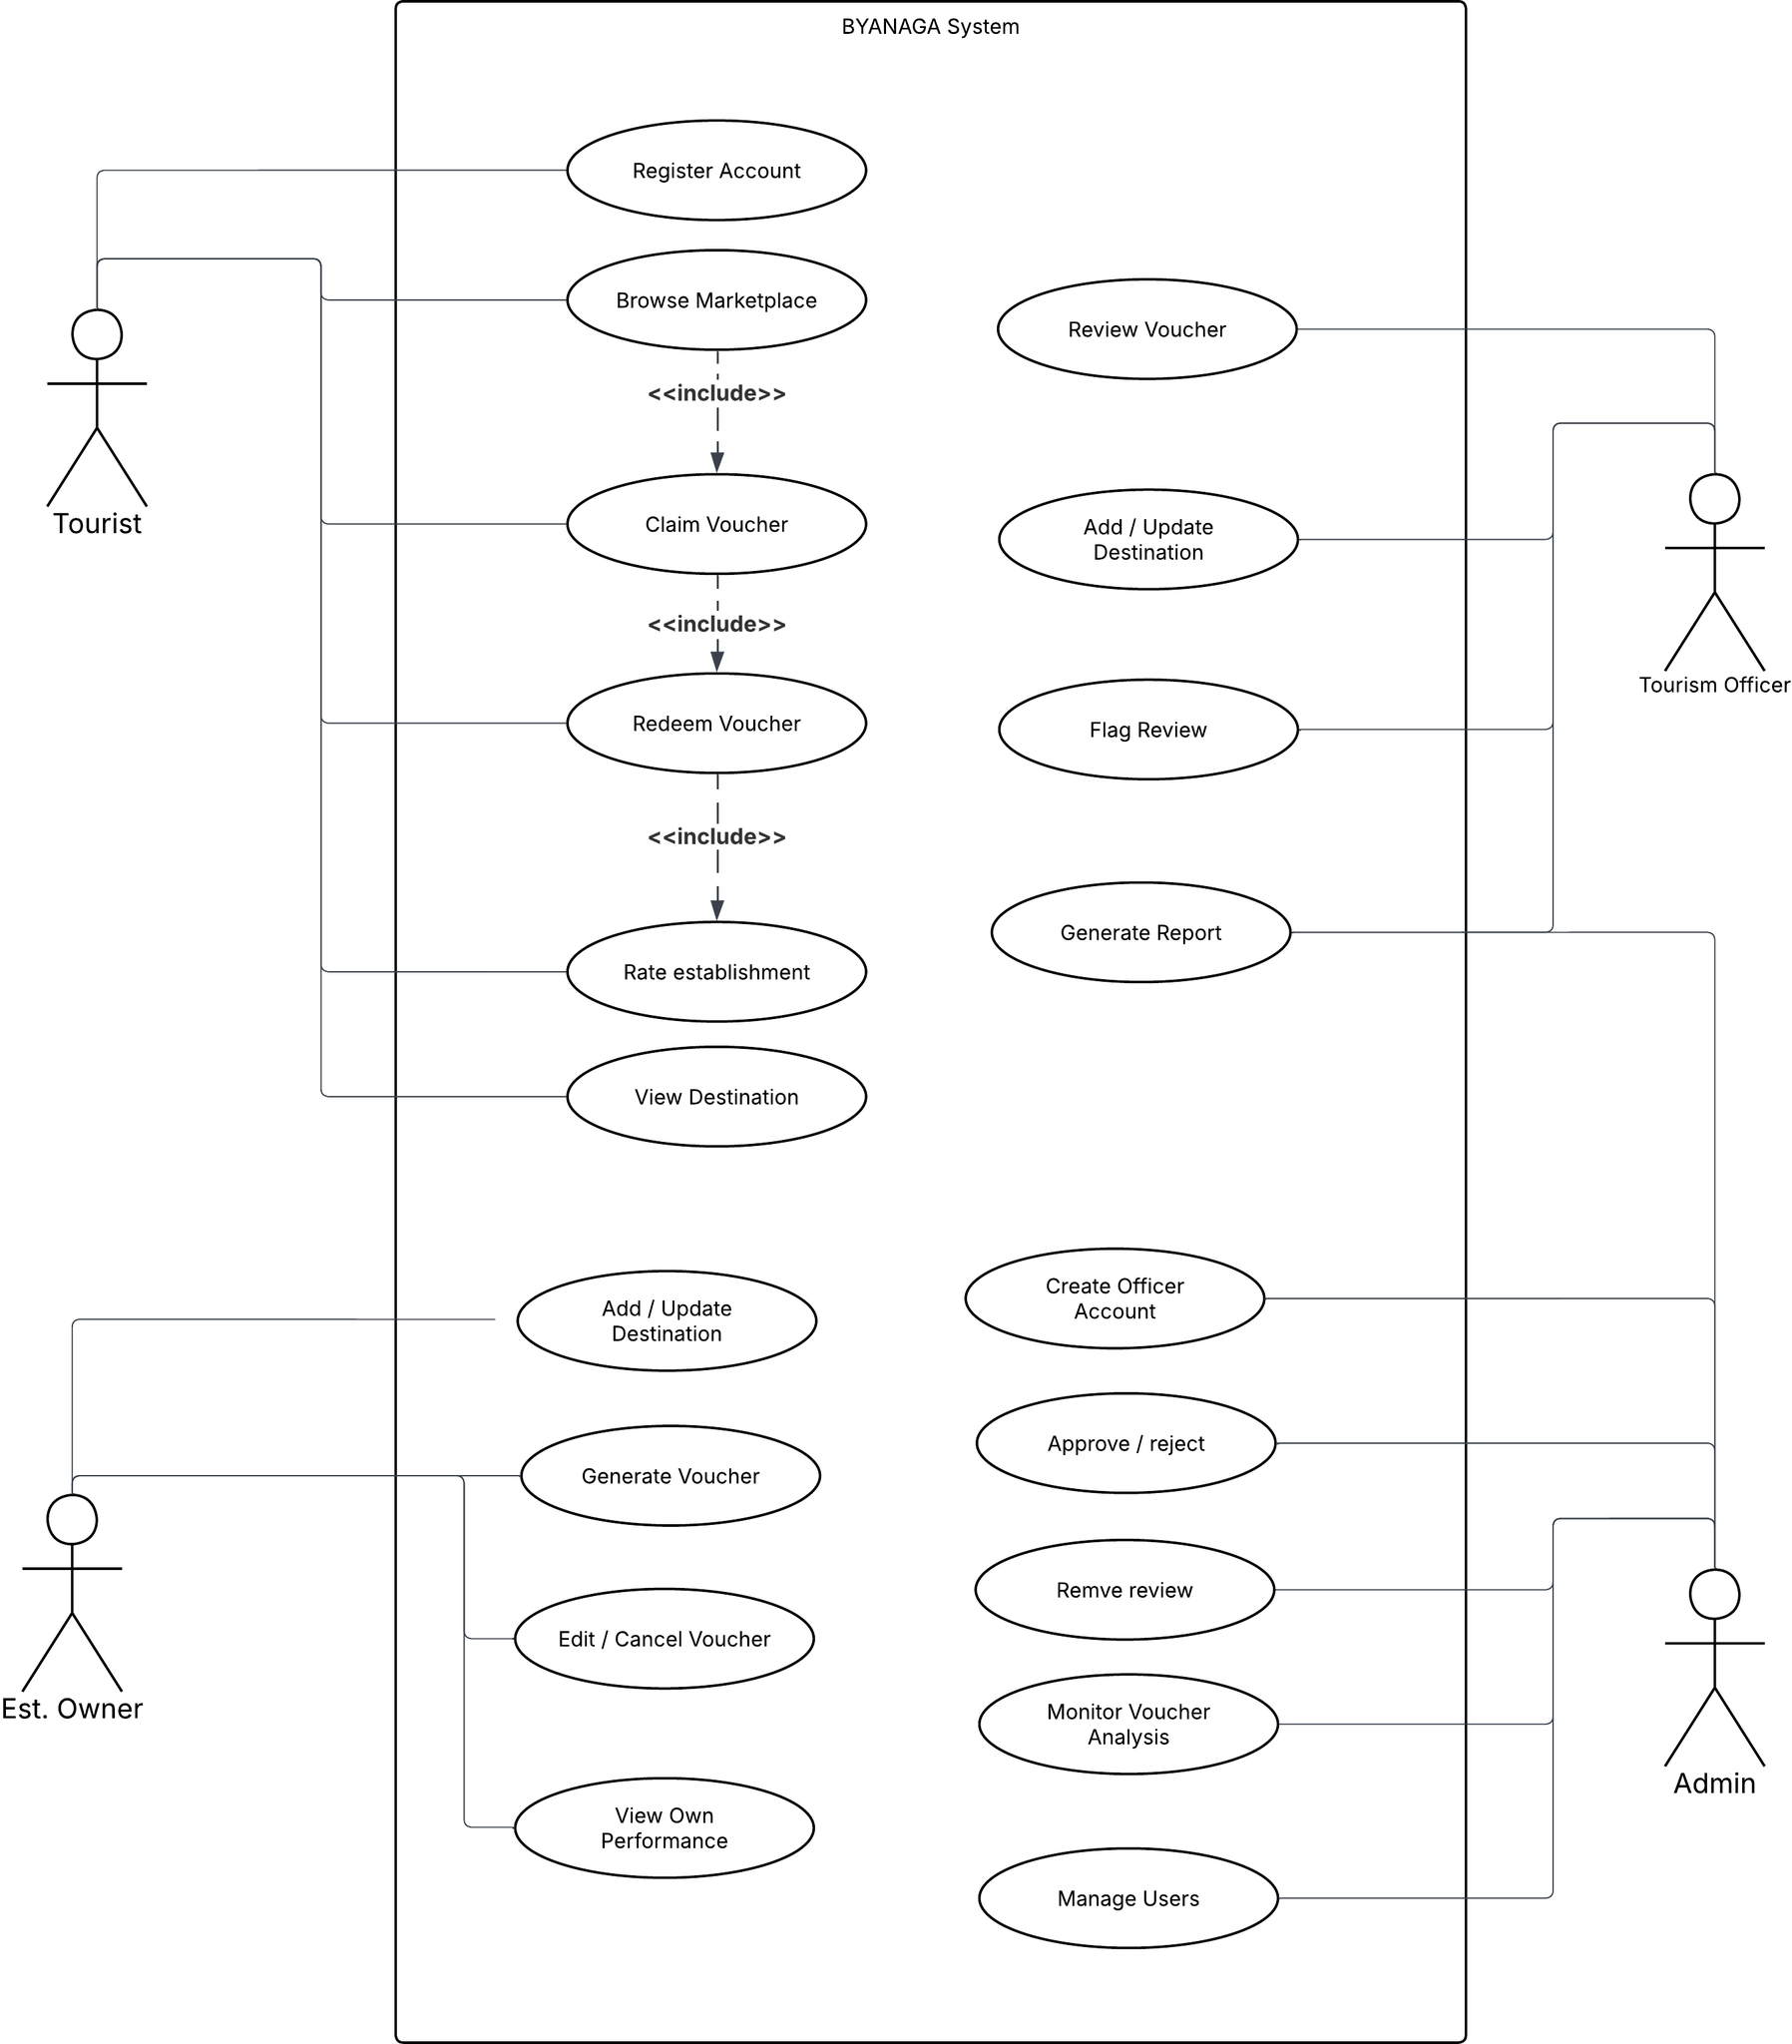
\includegraphics[width=\textwidth]{figures/UCD.png}
    \caption{Use Case Diagram of BYANAGA}
    \label{fig:use_case}
\end{figure}

According to the BYANAGA Use Case Diagram, there are four external actors involved in the process, including Tourist, Establishment Owner (Est. Owner), Tourism Officer, and Admin. These external actors have been associated with the functions that the system authorizes them to do.
The Tourist participates in six use cases. In order to get a personal account, he/she should Register Account. He/She is allowed to Browse Marketplace in order to check out all the vouchers and offers available, which also includes Claim Voucher through an include relationship. This implies that browsing comes before claiming a voucher since this is a compulsory function. The Claim Voucher also involves the function of Redeem Voucher, and thus the tourist should first redeem before he/she rates and reviews the establishment. The tourist may directly go for the activity of View Destination.
Establishment Owner has use case interaction with four other use cases. Establishment Owner has an ability to use Add or Update Destination use case to add information about the destination. Establishment Owner is able to use Generate Voucher to submit voucher creation request to an officer for approval. Establishment Owner can use Edit or Cancel Voucher use case in order to modify or cancel voucher submission prior to its examination by an officer. Moreover, Establishment Owner can track his performance by using View Own Performance use case.
Tourism Officer has use case interaction with four other use cases. Tourism Officer has an ability to use Review Voucher use case in order to examine voucher submission and make a decision about it either approving or sending back along with written revision recommendations. Tourism Officer uses Add or Update Destination use case with Establishment Owner. Tourism Officer is able to use Flag Review use case in order to escalate tourist review to the Administrator for further examination. Finally, Tourism Officer can generate reports in the form of PDF or CSV files.
The Administrator participates in five use cases. The Administrator may create an Officer Account by registering and assigning Tourism Officer users into the system. The Administrator can either approve or reject requests made by establishment owners who want to access the platform. The Administrator may remove Tourist Review for any reviews that are not in compliance with platform policies, as identified by the officer. The Administrator may manage Voucher Analysis to manage all voucher data analytics in the system. The Administrator may Manage Users, thereby creating, editing, suspending, or deactivating any account in the system.
The above diagram shows the system boundary for the BYANAGA system, what activities each actor must participate in, and the dependency between the different processes – especially the include dependency chain that starts from Browse Marketplace through Claim Voucher, Redeem Voucher, and eventually Rate Establishment.

\subsubsection{Data Flow Diagram}

\begin{figure}[H]
    \centering
    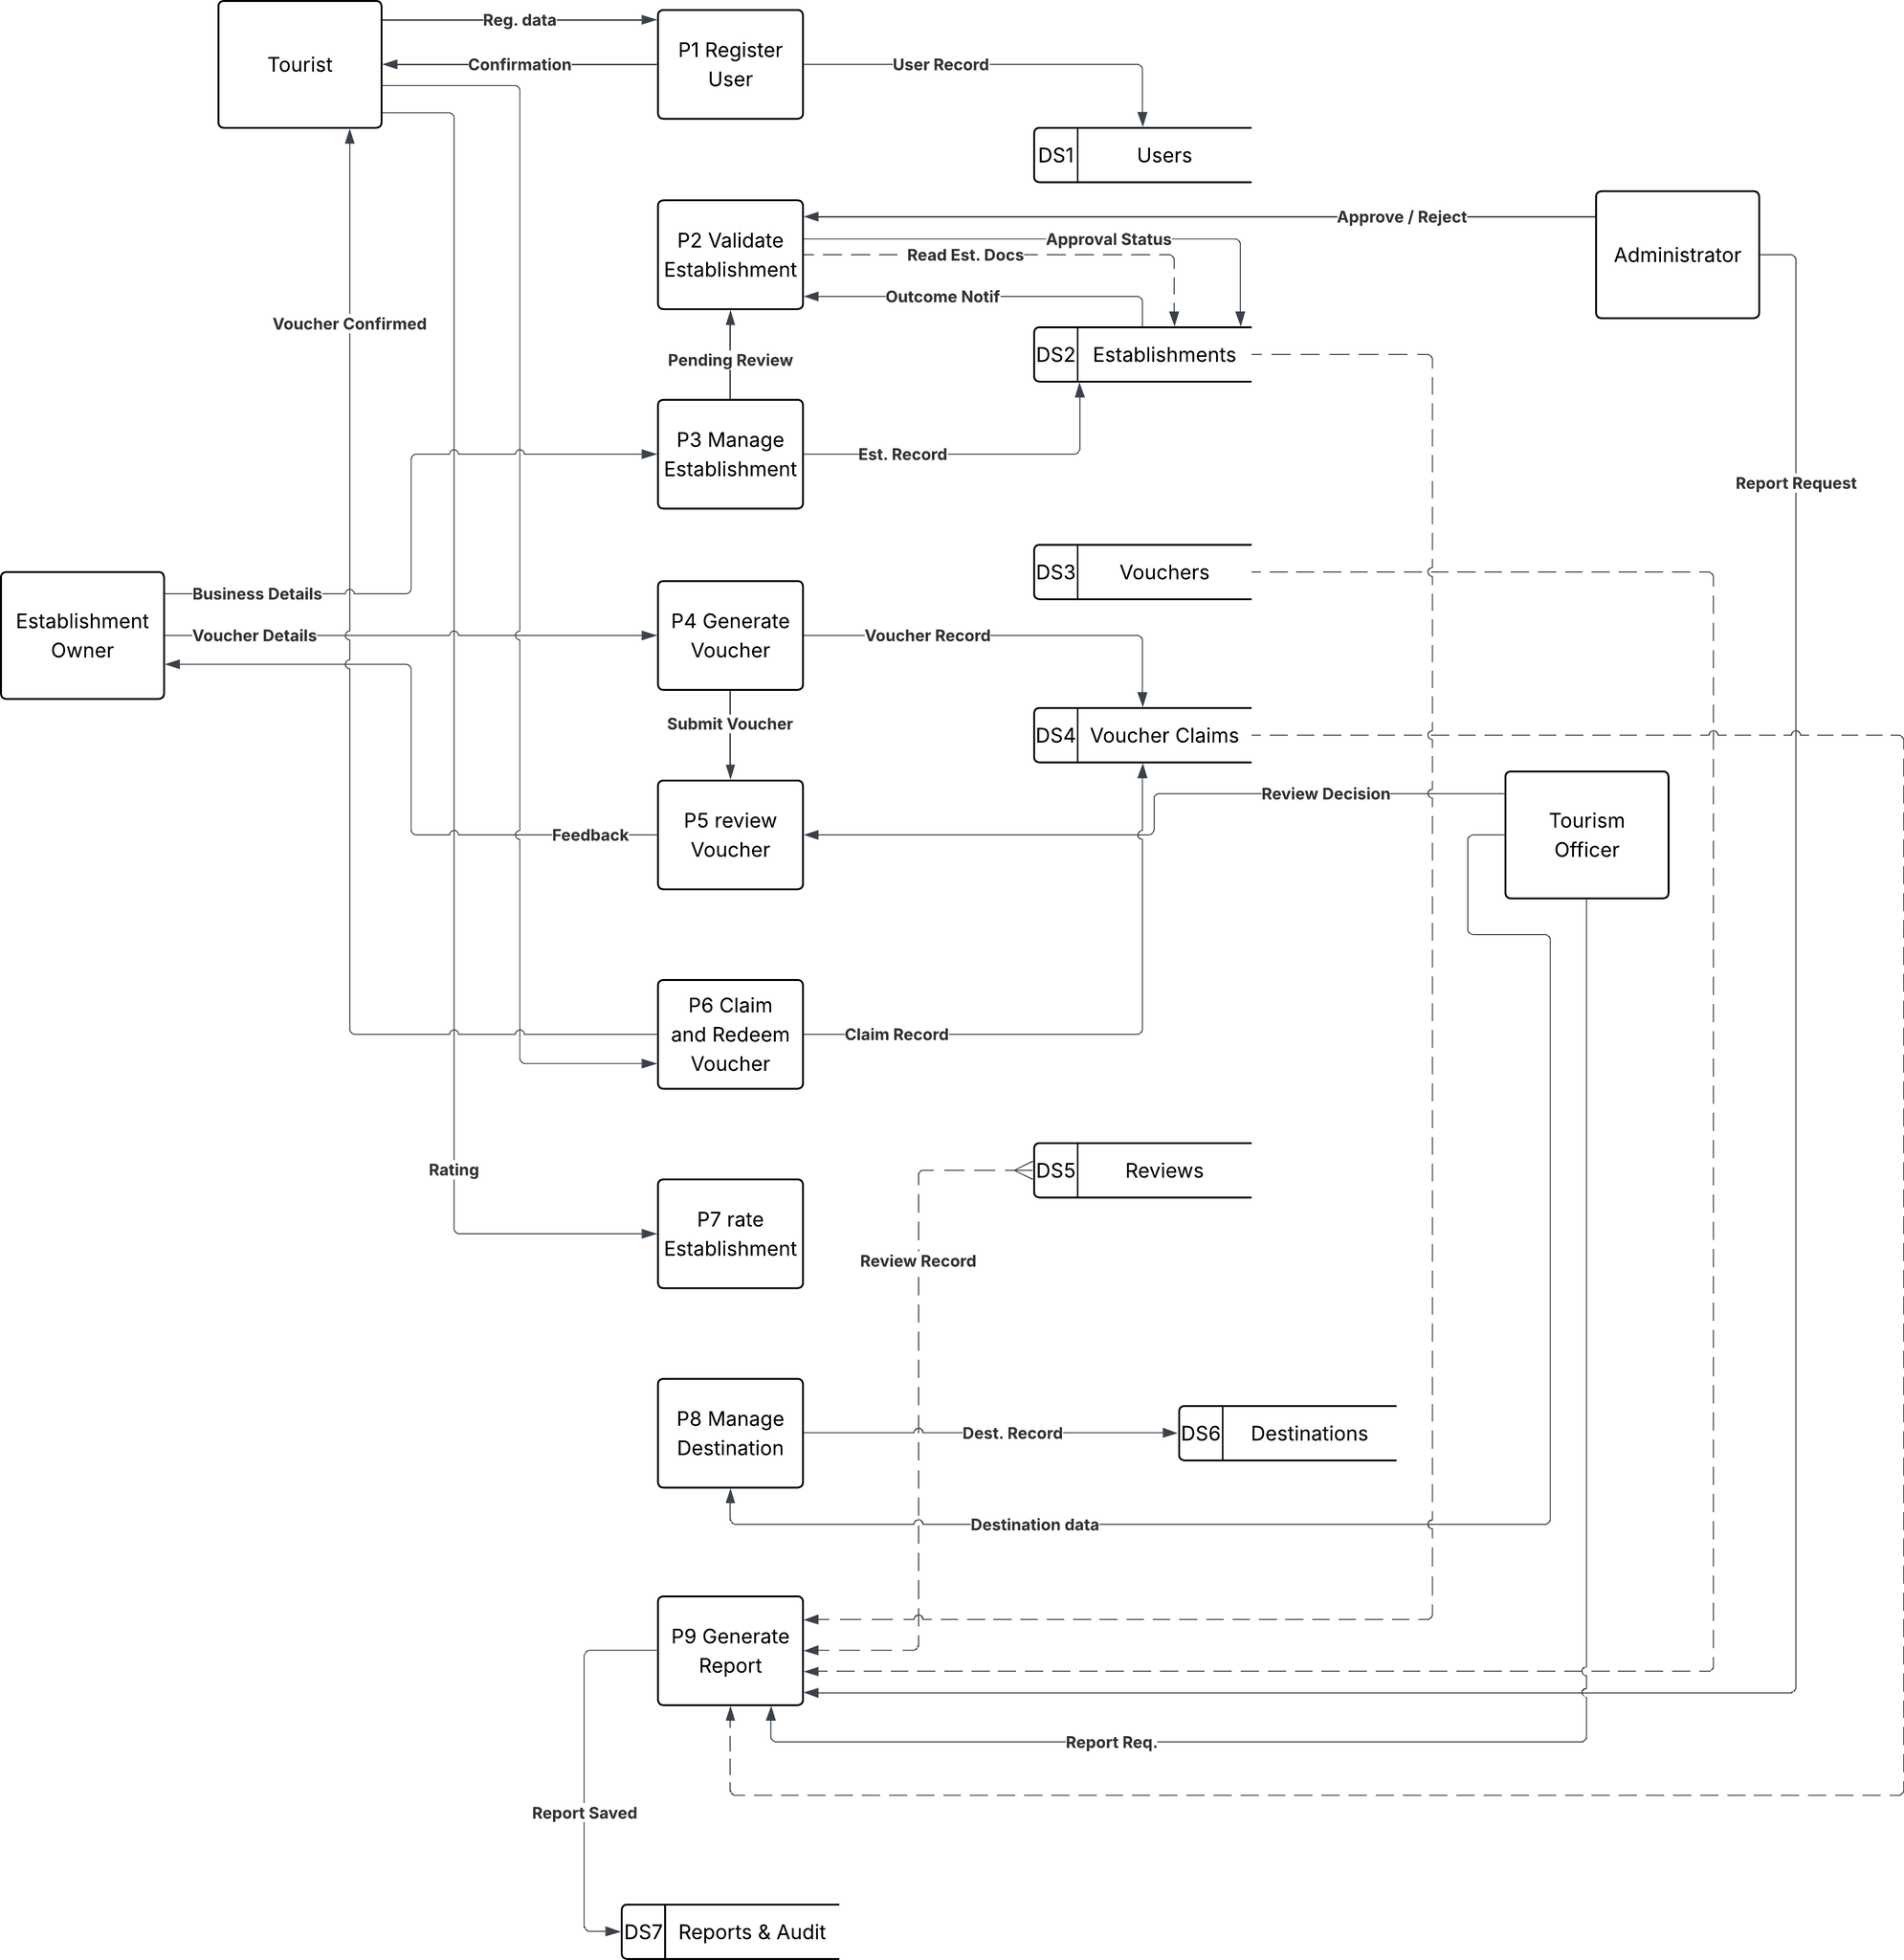
\includegraphics[width=\textwidth]{figures/DFDL1.png}
    \caption{Level 1 Data Flow Diagram of BYANAGA}
    \label{fig:dfd_level1}
\end{figure}

Data Flow Diagram Level 1 of BYANAGA extends the system through nine interrelated processes depicting how data flows between four entities external to the organization – Tourist, Establishment Owner, Tourism Officer, and Administrator – and seven data stores.
Process 1 entails registration of tourists and account storage in DS1 (Users). Process 2 deals with validation of establishments by the Administrator, where the results are saved in DS2 (Establishments). Process 3 enables authorized owners to make modifications on establishment details kept in DS2. Process 4 involves generation of vouchers by owners, which are recorded in DS3 (Vouchers). Process 5 deals with review of vouchers by Tourism Officers, with feedback provided to the owner. Process 6 involves recording of tourist vouchers and their redemption into DS4 (Voucher Claims). Process 7 deals with storing of tourist reviews and ratings in DS5 (Reviews). Process 8 involves management of destination record in DS6 (Destinations) by Tourism Officers. Process 9 deals with report generation involving collection of data from all data stores and saving the report in DS7 (Reports and Audit Trail).

\subsubsection{Business Process Modeling Notation (BPMN)}

\begin{figure}[H]
    \centering
    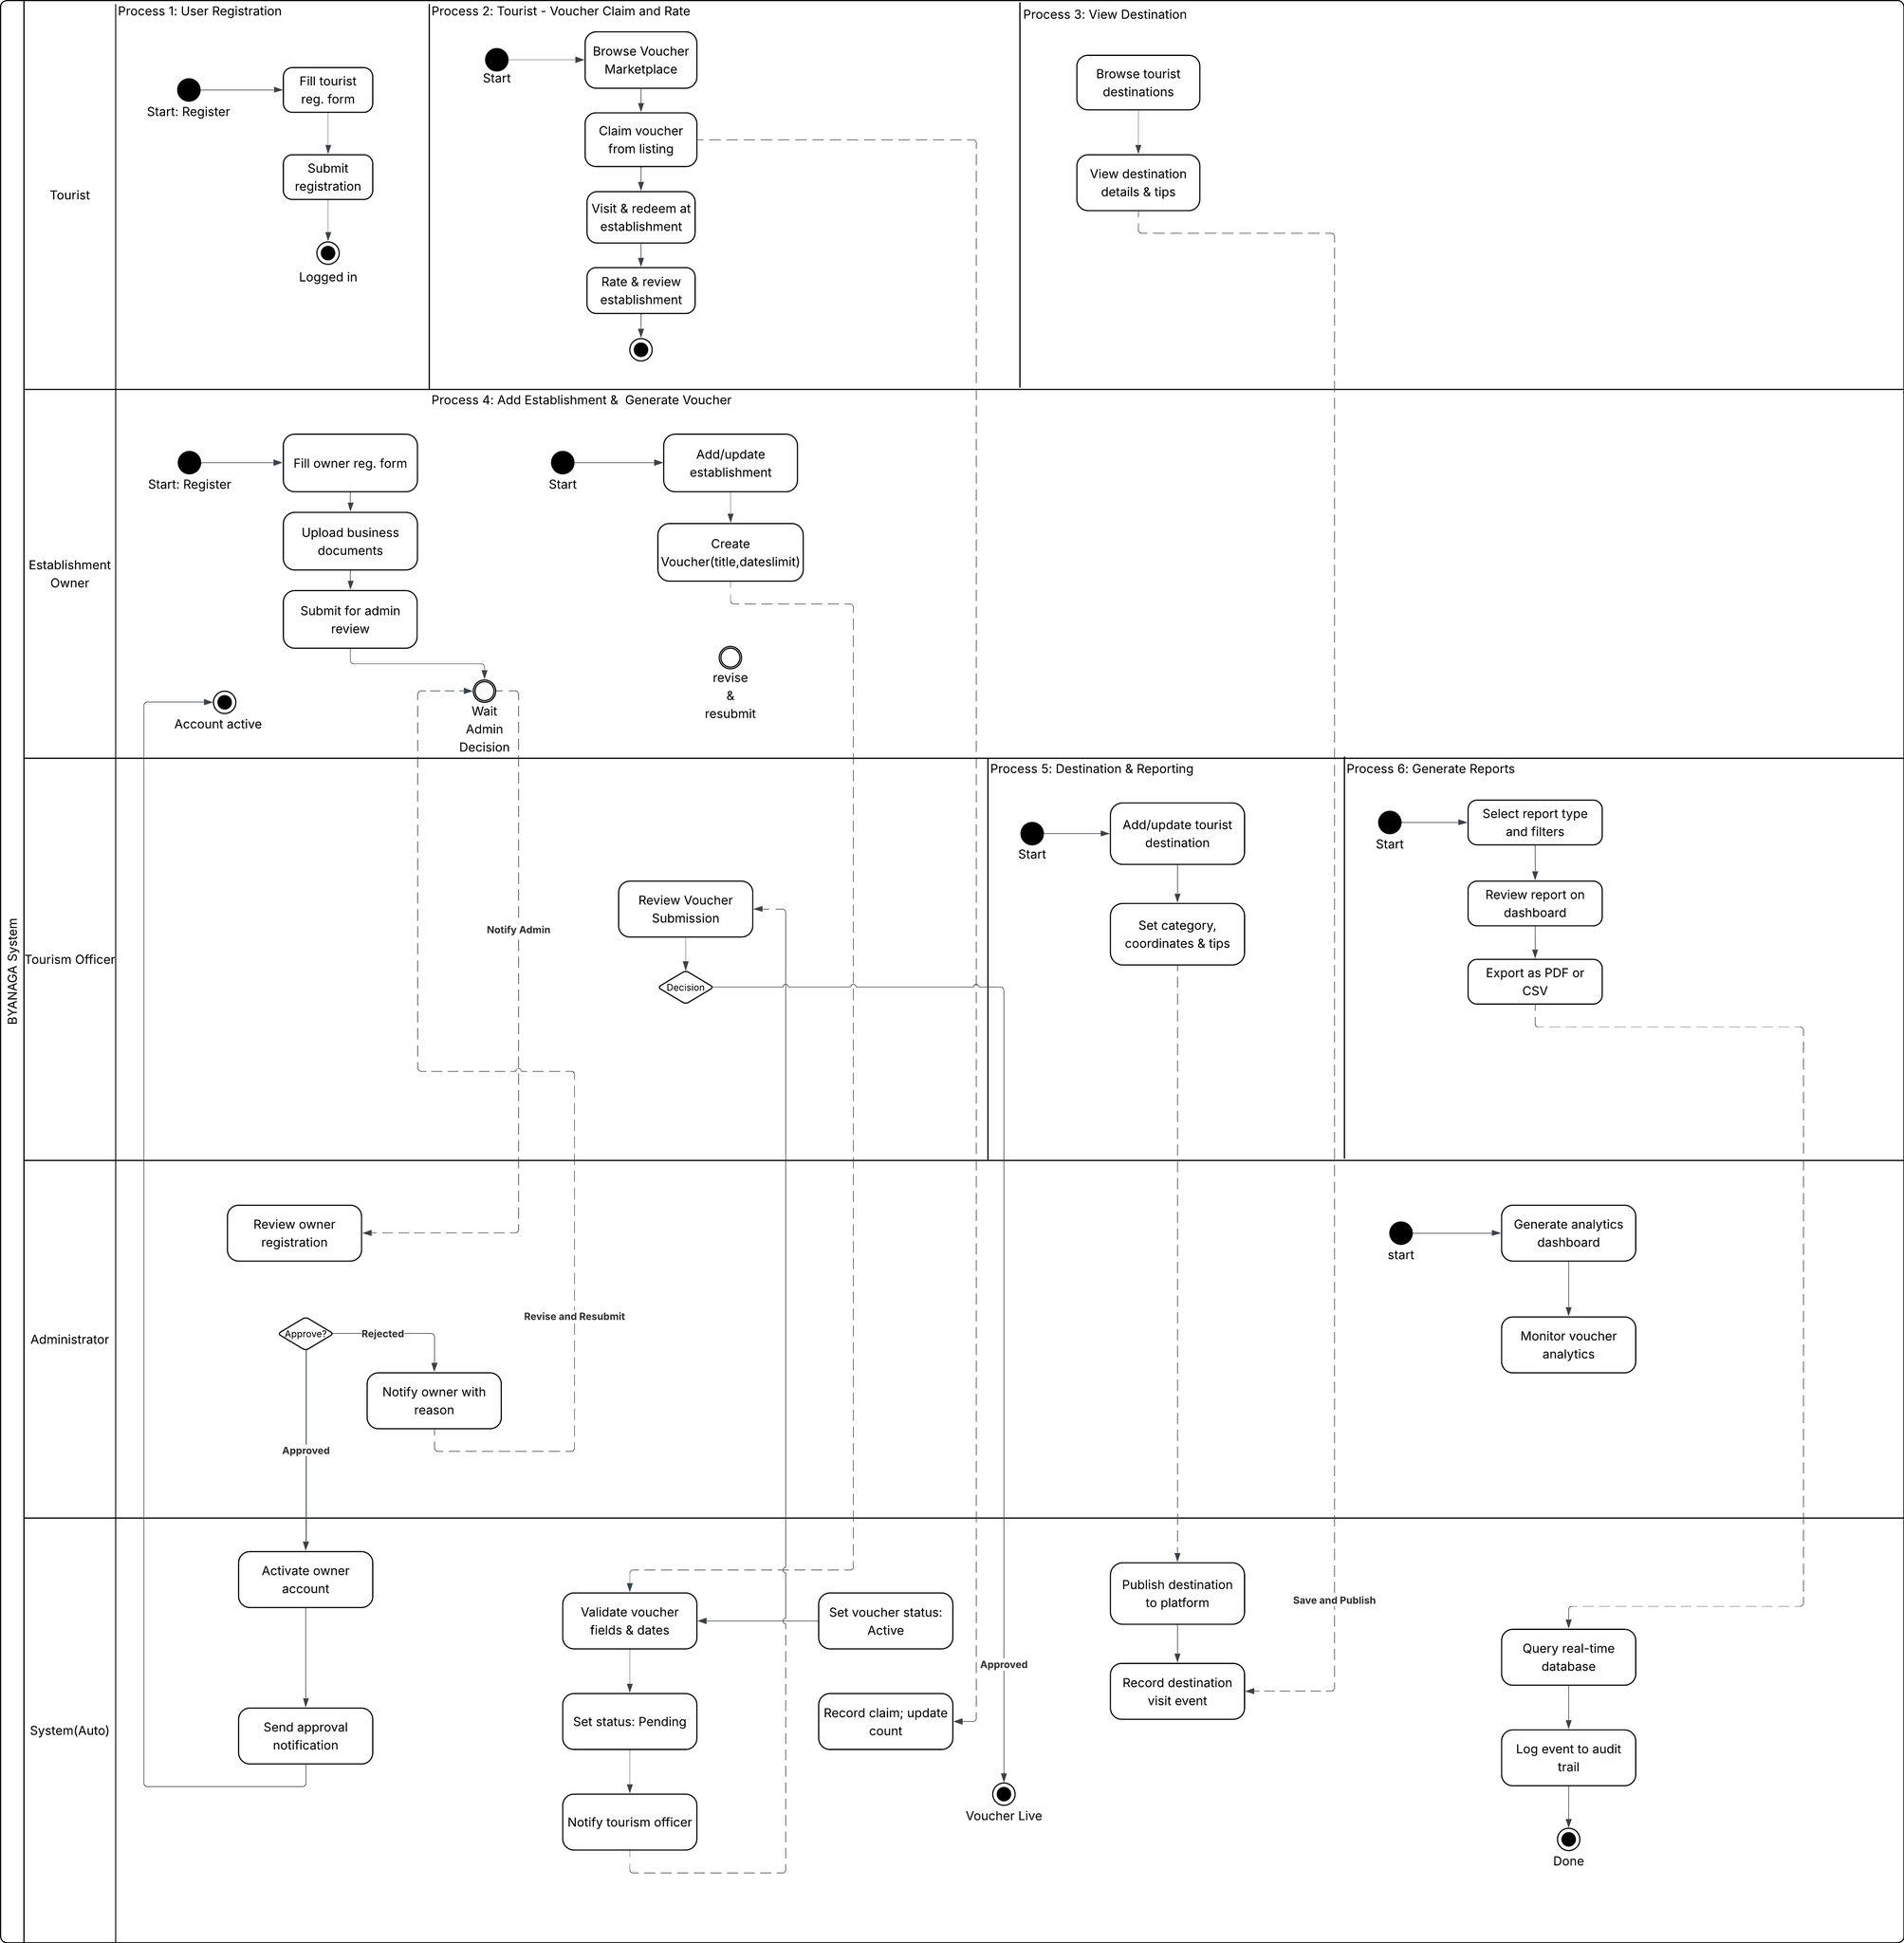
\includegraphics[width=\textwidth]{figures/BPMN.png}
    \caption{Business Process Modeling Notation}
    \label{fig:bpmn}
\end{figure}

The BPMN Diagram of BYANAGA presents the workflows from end to end of five roles: Tourist, Establishment Owner, Tourism Officer, Administrator, and the System through swimlanes, defining the responsibility of each role and how actions occur among these roles.
The swimlane of Tourist contains three processes, namely registration, voucher collection and redemption followed by rating of establishment, and exploration of tourist destinations. On the other hand, the swimlane of Establishment Owner contains processes such as registration of account with documents attached, establishment profile maintenance, and voucher creation involving modification and resubmission process. Furthermore, the Tourism Officer contains processes such as vouchers' review and approval, management of tourist destinations, and generation of report in PDF and CSV format. The Administrator involves in processes that include verification of the validity of establishments' registration, activation of account, and voucher dashboard management. Meanwhile, the System lane involves automation of actions such as notification, validation of voucher's field values, increment in claim number, documentation of redemptions, publication of destination, and log of audit trail.
Thus, through the diagram, it can be seen how the operation of BYANAGA is structured with the help of approval mechanism and automation process.

\subsubsection{Entity-Relationship Diagram}

\begin{figure}[H]
    \centering
    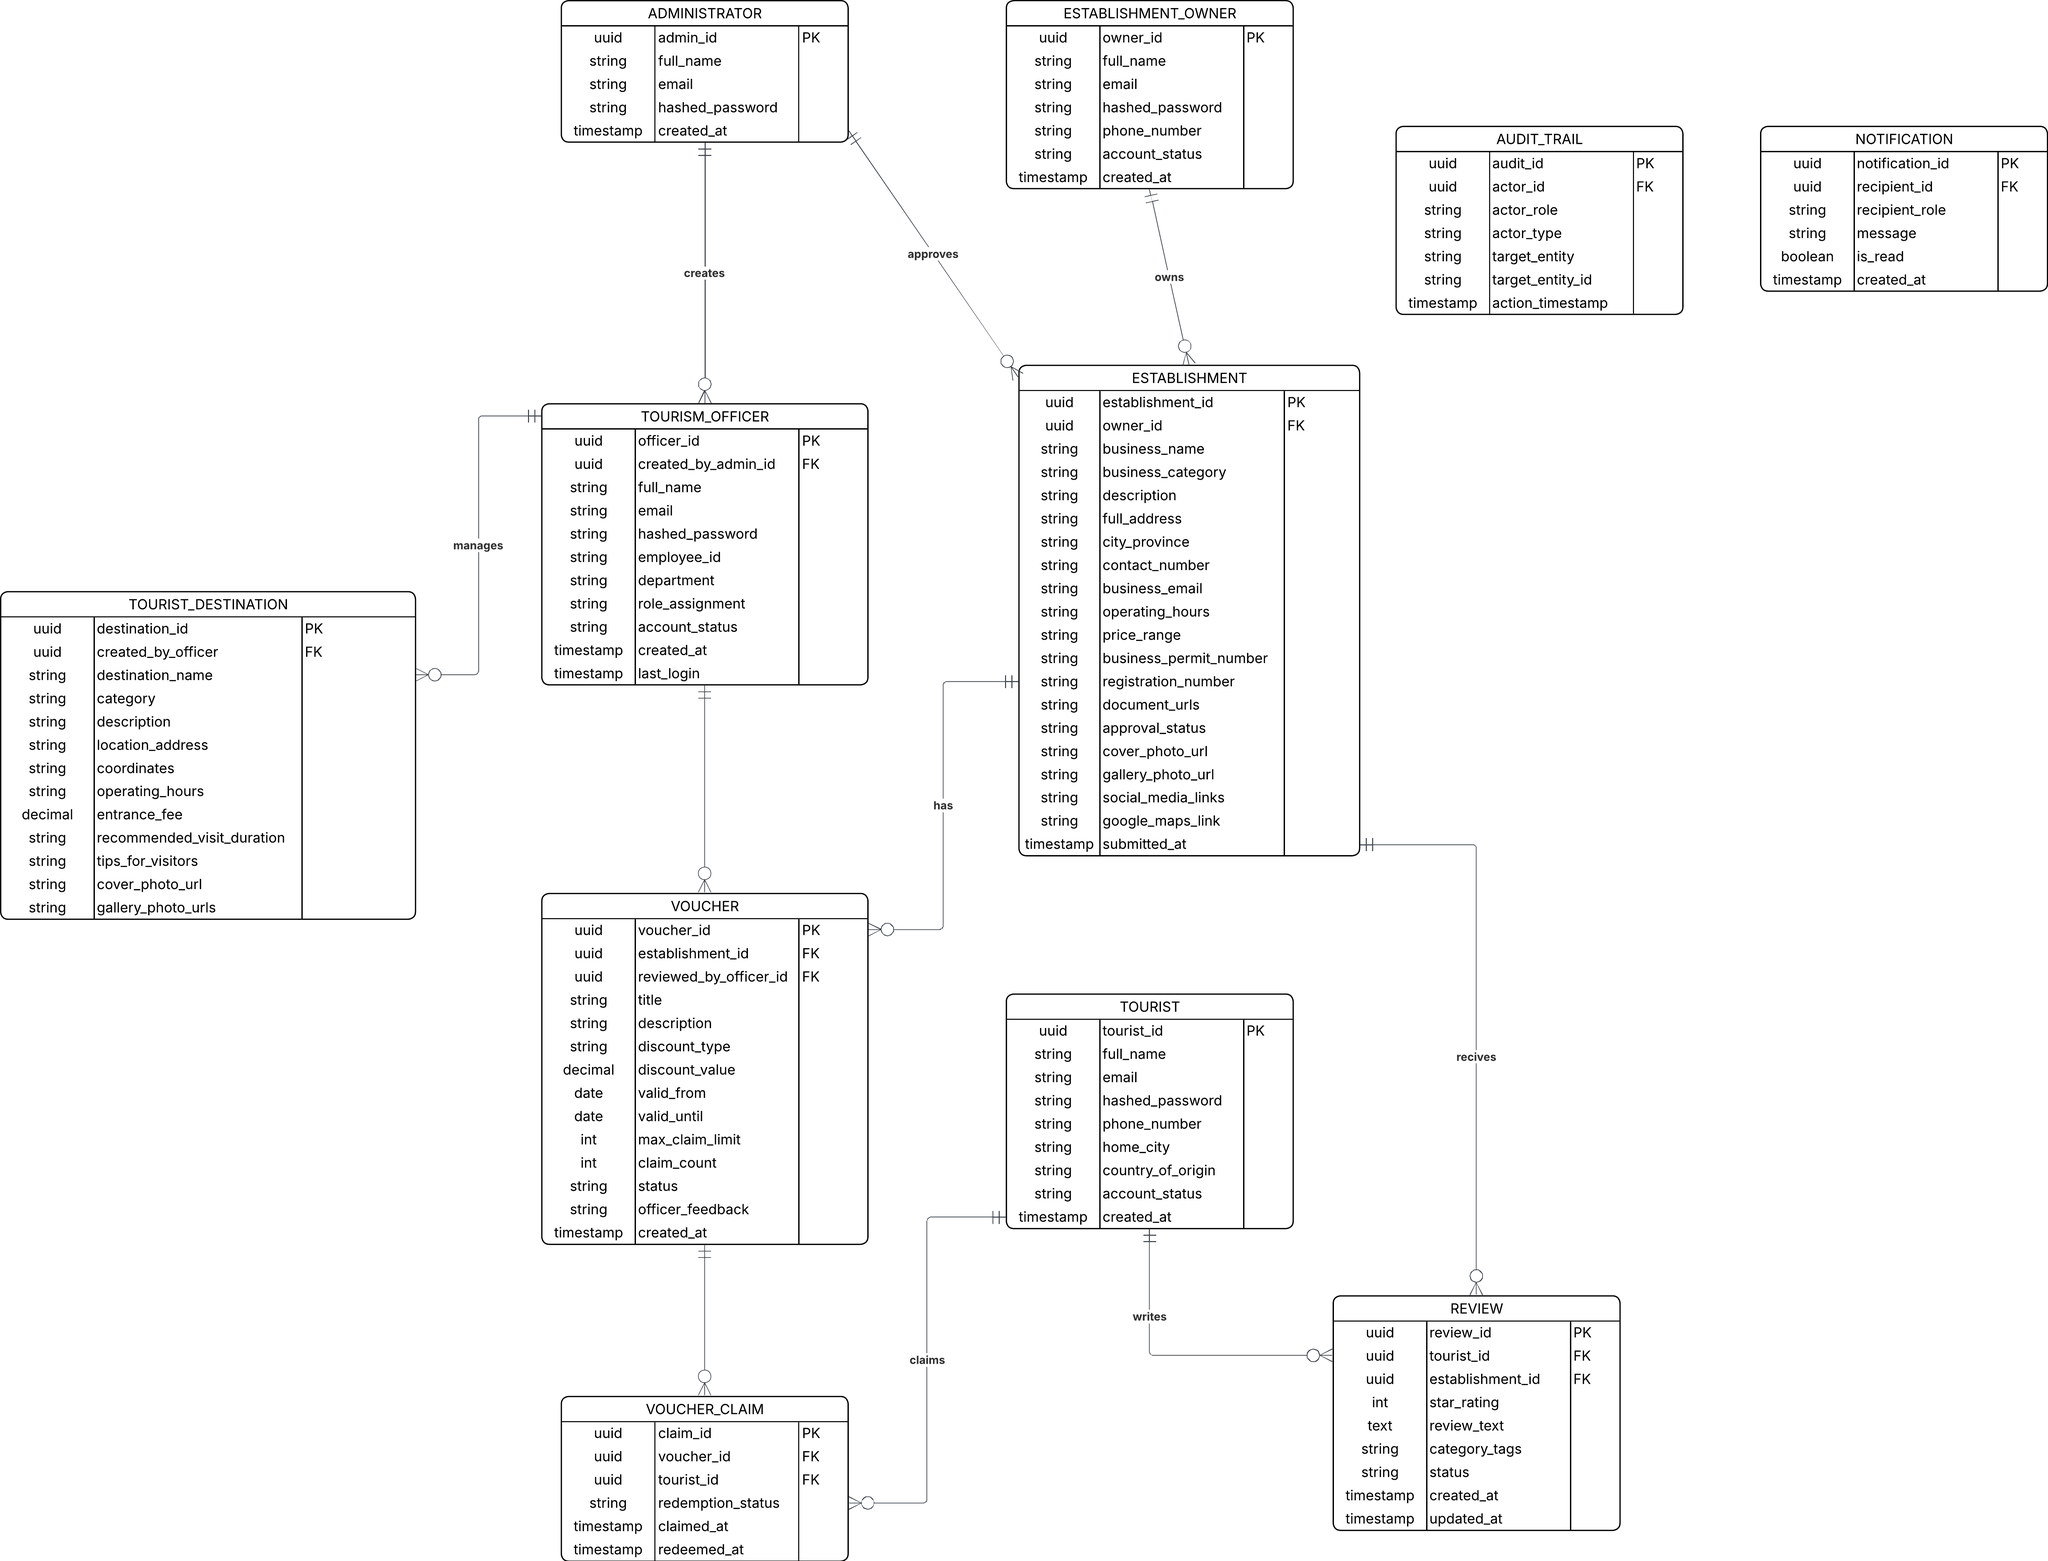
\includegraphics[width=\textwidth]{figures/ERD.png}
    \caption{Entity-Relationship Diagram of BYANAGA (Crow's Foot Notation)}
    \label{fig:erd}
\end{figure}

The Entity Relationship Diagram of BYANAGA describes the relational database through eleven core entities: Administrator, Tourism Officer, Establishment Owner, Establishment, Tourist Destination, Voucher, Tourist, Voucher Claim, Review, Notification, and Audit Trail.
The role of Administrators is to set up officer accounts and validate establishment entries. Tourism Officers are responsible for management of tourist destinations and review of vouchers. An Establishment Owner is associated with one or more Establishments, holding their names, categories, locations, permit number, validation status, and uploaded documents. Vouchers are tied to Establishments with discount information, expiration dates, number of claims possible, statuses, and officer remarks. Tourists claim their vouchers via the Voucher Claim, indicating the voucher's redemption and the timestamp. Reviews keep record of rating, message, and keywords left by tourists post-redeeming vouchers. Locations of Tourist Destinations contain the geographical information, coordinates, working hours, and travel tips managed by Officers. Notifications capture system messages sent out for particular users and roles. Audit Trail records all activities performed within the system along with its actor, action, target, and timestamp.
The ERD thus establishes the relational framework on which the proposed system functions.
    
\clearpage

%-----------------------------
% References
%-----------------------------

\clearpage

\printbibliography

\clearpage

\end{document}